\documentclass[output=paper,colorlinks,citecolor=brown]{langscibook} 
\ChapterDOI{10.5281/zenodo.22078583}

\author{Olav Mueller-Reichau\affiliation{University of Leipzig}}
\title{The morphosemantics of Russian aspect}  

\SetupAffiliations{mark style=none}

\abstract{Compositional semantic analyses of Slavic aspect face the challenge that no clear morphological exponents of perfective or imperfective can be identified on the verb. Against this background, the present article, concentrating on the case of Russian, pursues two goals. The first is to provide an overview of formal semantic analyses that answer the question of which parts of verbal morphology carry which mea\-ning. The second aim is to present a new formal semantic analysis, stated within the theoretical framework of discourse representation theory (DRT), which makes do with a single aspectual null operator. Unlike previous theories of this kind, the new approach relies on state change (rather than quantization) as the relevant lexical aspectual feature, and it presupposes time intervals (rather than time points) as relevant temporal units in the model. It is shown in detail how the new proposal can explain the range of (im)perfective readings identified in traditional Russian aspectology.}


\IfFileExists{../localcommands.tex}{
   \addbibresource{../localbibliography.bib}
   \usepackage{tabularx,multicol}
\usepackage{url}
\urlstyle{same}

 
\usepackage{langsci-optional}
\usepackage{langsci-lgr}
\usepackage{langsci-gb4e}

% ADDED BY VOLUME EDITORS

% \usepackage{langsci-osl} % macros specific to Open Slavic Linguistics; PLACED DIRECTLY IN localcommands.tex
\usepackage{siunitx}
\usepackage[linguistics]{forest}
% \usepackage{caption} %borik (?)
\usepackage{pifont} %geist

% 08_muellerreichau

% \usepackage{caption}
\usepackage{subcaption}
\usepackage{cleveref}

\usepackage{drs}
\usepackage{diagbox}

% 09_simik

\usepackage{multirow}
\usepackage{tabto}

% 10_stegovec

\usetikzlibrary{arrows,patterns}
\usepackage{listings}
% \usepackage{multirow}

% 01_gehrke-simik

% \usepackage{comment}

% 13_wagiel

% \usepackage{pifont} % for checkmarks (\ding{51}, \ding{55})


\usepackage{langsci-branding}

   % \newcommand*{\orcid}{}


\makeatletter
\let\thetitle\@title
\let\theauthor\@author
\makeatother

\newcommand{\togglepaper}[1][0]{
   \bibliography{../localbibliography}
   \papernote{\scriptsize\normalfont
     \theauthor.
     \titleTemp.
     To appear in:
     E. Di Tor \& Herr Rausgeberin (ed.).
     Booktitle in localcommands.tex.
     Berlin: Language Science Press. [preliminary page numbering]
   }
   \pagenumbering{roman}
   \setcounter{chapter}{#1}
   \addtocounter{chapter}{-1}
}

\newbool{bookcompile}
\booltrue{bookcompile}
\newcommand{\bookorchapter}[2]{\ifbool{bookcompile}{#1}{#2}}

\AtBeginDocument{\nogltOffset} %removes extra spacing before trans line in examples - SPECIFIC TO OPEN SLAVIC LINGUISTICS, PREVIOUSLY AGREED UPON


%%%%%%%%%%%%%%%%%%%%%%%%%%%%%%%%%%%%%%%%%%%%%%%%%%%%%%%%%%%%%%%%%%%%%
%%      File: langsci-osl.sty
%%    Author: Radek Simik and Language Science Press (http://langsci-press.org)
%%      Date: 2019-02-18
%%   Purpose: This file contains macros for the Open Slavic Linguistics at Language Science Press series and is included 
%%            into langscibook.cls
%%  Language: LaTeX
%%   Licence: 
%%%%%%%%%%%%%%%%%%%%%%%%%%%%%%%%%%%%%%%%%%%%%%%%%%%%%%%%%%%%%%%%%%%%%

% FIXING GRAY

\definecolor{lsDOIGray}{cmyk}{0,0,0,0.45}

% PACKAGES REQUIRED

\RequirePackage{relsize}
\RequirePackage{stmaryrd}
\RequirePackage{array}
\RequirePackage{tabularx}

% % KEYWORDS

% \newcommand{\keywords}[1]{\noindent\textbf{Keywords:} {#1}}

% SEMANTICS MACROS - GENERAL FOR ALL PAPERS

\newcommand{\sib}[1]{$\llbracket${#1}$\rrbracket$} % = semantic interpretation brackets; puts text into double square brackets
\newcommand{\stb}[1]{\langle{#1}\rangle} % = semantic type brackets; puts stuff into semantic type brackets; necessary to use in the form $\st{}$
\newcommand{\cnst}[1]{\textsf{\relsize{-1}\MakeUppercase{#1}}} %creates sans-serif small-caps, used for typesetting logical constants which have no other appropriate symbols (such as Greek letters)

% MINUS HSPACE MACRO

\newcommand{\minsp}[1]{#1\hspace{-2.5pt}} % use for non-glossed elements in glossed examples (typically stars, brackets, slashes, ...)

% CITATION MACROS

\newcommand{\citeposst}[1]{\citeauthor{#1}'s (\citeyear{#1})} % produces Chomsky's (1995)
\newcommand{\citeposstpg}[2]{\citeauthor{#1}'s (\citeyear[#2]{#1})} % produces Chomsky's (1995: page)
\newcommand{\citepossalt}[1]{\citeauthor{#1}'s \citeyear{#1}} % produces Chomsky's 1995
\newcommand{\citepossaltpg}[2]{\citeauthor{#1}'s \citeyear[#2]{#1}} % produces Chomsky's 1995: page

% BARPLOT

\usepackage{pgfplots}
\pgfplotsset{compat=1.18} 
\newcommand{\barplot}[5]{%
  \begin{tikzpicture}
    \begin{axis}[
	xlabel={#1},  
	ylabel={#2}, 
	axis lines*=left, 
        width  = {#3\textwidth},
	height = .3\textheight,
    	nodes near coords, 
	xtick=data,
	x tick label style={},  
	ymin=0,
	symbolic x coords={#4},
	]
	\addplot+[ybar,lsRichGreen!80!black,fill=lsRichGreen] plot coordinates {
	    #5
	}; 
    \end{axis} 
  \end{tikzpicture} 
}



%%%%%%%%%%%%%%%%%%%%%%%%%%%
%%% 04_filip %%%

% \newcommand{\mC}[1]{\multicolumn{1}{c}{#1}} % multicolumn with a single column; ALREADY DEFINED

\usetikzlibrary{arrows, arrows.meta}
\usetikzlibrary{positioning, decorations, 
                decorations.pathreplacing, calligraphy}

%%%%%%%%%%%%%%%%%%%%%%%%%
%%% 08_muellerreichau %%%

\captionsetup[subfigure]{subrefformat=simple,labelformat=simple}
\renewcommand\thesubfigure{(\alph{subfigure})}

%%%%%%%%%%%%%%%%%%%%%%%%%%%
%%% 09_simik

\newcommand{\citepossts}[1]{\citeauthor{#1}' (\citeyear{#1})} % produces Rawlins' (2008)
\newcommand{\citepossalts}[1]{\citeauthor{#1}' \citeyear{#1}} % produces Rawlins' 2008


%%%%%%%%%%%%%%%%%%%%%%%%%%%%%%%
%%% 10_stegovec

\newcommand{\poscite}[1]{\citeauthor{#1}'s (\citeyear{#1})}

%extra commands
\newcommand{\fst}{\textsc{1p}}
\newcommand{\snd}{\textsc{2p}}
\newcommand{\trd}{\textsc{3p}}
\newcommand{\refl}{\textsc{refl}}
\newcommand{\excl}{\textsc{excl}}
\newcommand{\incl}{\textsc{incl}}
\newcommand{\sg}{\textsc{sg}}
\newcommand{\pl}{\textsc{pl}}
\newcommand{\dl}{\textsc{dl}}
\newcommand{\fem}{\textsc{f}}
\newcommand{\masc}{\textsc{m}}
\newcommand{\neut}{\textsc{n}}
\newcommand{\ImpCl}{IMPERATIVE}


\newcommand{\tikzmark}[1]{\tikz[overlay,remember picture] \node (#1) {};}
\forestset{M/.style={
		for tree={s sep=5mm, inner sep=0.5pt, l=5mm,
			calign=fixed edge angles,
			calign primary angle=-65,
			calign secondary angle=65},
	},
	Mid/.style={
		for tree={s sep=0mm, inner sep=0pt, l=0mm,
			calign=fixed edge angles,
			calign primary angle=-62.5,
			calign secondary angle=62.5},
	},
	word/.style={before typesetting nodes={content=\emph{##1}},
		no edge,l=0,for parent={l sep=0}},
	feat/.style={before typesetting nodes={content={{[}##1{]}}},
		no edge,l=0,for parent={l sep=0}},
	feat2/.style={before typesetting nodes={content={##1}},
		no edge,l=0,for parent={l sep=0}},
	llap/.style={
		tikz+={%
			\edef\forest@temp{\noexpand\node[\option{node options},
				anchor=base east,at=(.base east)]}%
			\forest@temp{#1\phantom{\option{environment}}};
		}
	},
	rlap/.style={
		tikz+={%
			\edef\forest@temp{\noexpand\node[\option{node options},
				anchor=base west,at=(.base west)]}%
			\forest@temp{\phantom{\option{environment}}#1};
		}
	}
}

\makeatletter
\newcommand{\coloruline}[2]{%
	\newcommand\temp@reduline{\bgroup\markoverwith
		{\textcolor{#1}{\rule[-0.5ex]{2pt}{0.4pt}}}\ULon}%
	\temp@reduline{#2}%
}

\newcommand{\coloruuline}[2]{%
	\UL@protected\def\temp@uuline{\leavevmode \bgroup
		\UL@setULdepth
		\ifx\UL@on\UL@onin \advance\ULdepth2.8\p@\fi
		\markoverwith{\textcolor{#1}{\lower\ULdepth\hbox
				{\kern-.03em\vbox{\hrule width.2em\kern1\p@\hrule}\kern-.03em}}}%
		\ULon}%
	\temp@uuline{#2}%
}

\newcommand{\coloruwave}[2]{%
	\UL@protected\def\temp@uwave{\leavevmode \bgroup 
		\ifdim \ULdepth=\maxdimen \ULdepth 3.5\p@
		\else \advance\ULdepth2\p@ 
		\fi \markoverwith{\textcolor{#1}{\lower\ULdepth\hbox{\sixly \char58}}}\ULon}
	\font\sixly=lasy6 % does not re-load if already loaded, so no memory drain.
	\temp@uwave{#2}%
}
\makeatother

%%%%%%%%%%%%%%%%%
%%% 13_wagiel %%%

\newcommand\irregularcircle[2]{% radius, irregularity
  \pgfextra {\pgfmathsetmacro\len{(#1)+rand*(#2)}}
  +(0:\len pt)
  \foreach \a in {10,20,...,350}{
    \pgfextra {\pgfmathsetmacro\len{(#1)+rand*(#2)}}
    -- +(\a:\len pt)
  } -- cycle
}


% IF POSSIBLE, CAN WE USE THIS SETTING JUST FOR 13_wagiel?

% \forestset{
% default preamble={for tree={s sep=10mm, inner sep=0, l=0}},
% fairly nice empty nodes/.style={
%         delay={where content={}{shape=coordinate,
%               for siblings={anchor=north}}{}},
% for tree={s sep=4mm}},
% }

   %% hyphenation points for line breaks
%% Normally, automatic hyphenation in LaTeX is very good
%% If a word is mis-hyphenated, add it to this file
%%
%% add information to TeX file before \begin{document} with:
%% %% hyphenation points for line breaks
%% Normally, automatic hyphenation in LaTeX is very good
%% If a word is mis-hyphenated, add it to this file
%%
%% add information to TeX file before \begin{document} with:
%% %% hyphenation points for line breaks
%% Normally, automatic hyphenation in LaTeX is very good
%% If a word is mis-hyphenated, add it to this file
%%
%% add information to TeX file before \begin{document} with:
%% \include{localhyphenation}
\hyphenation{
    par-a-digm
    Cart-wright %filip
    Truswell %docekal
    Shcher-bi-na %simik
    Mün-chen %gehrke
    Mo-ni-ka %gehrke
    spi-sov-né %gehrke
    li-te-ra-tur-no-go %gehrke
    russ-koj %gehrke
    so-ver-šen-no-go %gehrke
    russ-kom %gehrke
    sla-vjan-sko-mu %gehrke
    Zeit-schrift %gehrke
    Na-ta-sha %gehrke
    Zu-stands-pas-siv %gehrke
    Um-gangs-spra-che %gehrke
    Bra-so-vea-nu %geist
}

\hyphenation{
    par-a-digm
    Cart-wright %filip
    Truswell %docekal
    Shcher-bi-na %simik
    Mün-chen %gehrke
    Mo-ni-ka %gehrke
    spi-sov-né %gehrke
    li-te-ra-tur-no-go %gehrke
    russ-koj %gehrke
    so-ver-šen-no-go %gehrke
    russ-kom %gehrke
    sla-vjan-sko-mu %gehrke
    Zeit-schrift %gehrke
    Na-ta-sha %gehrke
    Zu-stands-pas-siv %gehrke
    Um-gangs-spra-che %gehrke
    Bra-so-vea-nu %geist
}

\hyphenation{
    par-a-digm
    Cart-wright %filip
    Truswell %docekal
    Shcher-bi-na %simik
    Mün-chen %gehrke
    Mo-ni-ka %gehrke
    spi-sov-né %gehrke
    li-te-ra-tur-no-go %gehrke
    russ-koj %gehrke
    so-ver-šen-no-go %gehrke
    russ-kom %gehrke
    sla-vjan-sko-mu %gehrke
    Zeit-schrift %gehrke
    Na-ta-sha %gehrke
    Zu-stands-pas-siv %gehrke
    Um-gangs-spra-che %gehrke
    Bra-so-vea-nu %geist
}

   \boolfalse{bookcompile}
   \togglepaper[8]%%chapternumber
}{}

\begin{document}

\maketitle

\section{Introduction} 
A lot of literature has been devoted to the form and function of Russian verbal aspect.\footnote{This chapter is about theories on Russian aspect only. Whether and in how far the results of the discussion presented below carry over to other Slavic languages remains to be seen. Although the aspectual systems of the Slavic languages resemble each other from a coarse-grained perspective, they differ in many relevant details. Inner-Slavic aspectual variation can be found in semantics as well as in morphosyntax (e.g. \citealt{Dickey2000}, \citealt{Petruchina12}).} Let me therefore emphasize that in this  
chapter, I will be concerned with the relationship between morphology and semantics of Russian aspect exclusively from a compositional semantic perspective. 
The following discussion will concentrate only on studies that approach the topic from this theoretical perspective. Even with this confinement, such a survey must necessarily be selective.  

%The form of a Slavic verb determines the aspectual value of the sentence in which it appears as perfective or imperfective. Polyaspectual verb forms, i.e. forms that allow for usage in perfective as well as imperfective contexts, are the exception rather than the rule.     

Within formal (compositional) semantics, Russian aspect is usually modelled as an operation over verbal meanings. Approaches disagree as to whether the syntactic constituent carrying the ``verbal meaning'' is a VP or a V (see \citealt{Rothstein20} for recent discussion). Another parameter with respect to which theories differ from each other relates to morphology. As is well known, there are no uncontroversial perfective or imperfective morphemes in Russian, that is to say, there are no necessary and sufficient markers of perfective or imperfective meaning.\footnote{To the exception of semelfactive \textit{nu}, from which I abstract away here.} Prefixes, which are not infrequently associated with perfectivity, appear also in imperfective forms (\ref{morfa}), and the secondary imperfective suffix, which seems to suggest itself as exponent of imperfectivity, shows up in perfective forms as well (\ref{morfb}).

\ea\label{morf}
\ea {ot}kryt'\textsuperscript{PFV} `open' -- {ot}kryvat'\textsuperscript{IPFV} `open'\label{morfa}
\ex otkry{va}t'\textsuperscript{IPFV} -- zaotkry{va}t'\textsuperscript{PFV} `start opening'\label{morfb}
\z\z

\noindent From a formal semantic perspective, the frequently made assumption that verbal prefixes mark perfectivity faces the problem of how to deal with imperfective verbs like \textit{otkryvat'} in (\ref{morf}). To claim for these that the prefix does not introduce the perfective meaning that it carries in \textit{otkryt'} would run against basic assumptions of compositionality. 
This problem is maybe even more apparent in aspectual triplets such as (\ref{tripl}):

\ea\label{tripl}
\ea čitat'\textsuperscript{IPFV} `read' -- {pro}čitat'\textsuperscript{PFV} `read (through)'
\ex {pro}čitat'\textsuperscript{PFV} -- {pro}čit{yva}t'\textsuperscript{IPFV} `read (through)'
\z\z

\largerpage
\noindent If one wanted to maintain that prefixes introduce perfective operators, one would have to come up with a semantics for the imperfective suffix YVA that, operating on a perfective meaning as input, somehow gets rid of the completedness entailment added by the prefix beforehand.\footnote{I use ``YVA'' as a handy term to refer to the operator the application of which manifests itself morphologically as suffixation. Subject to laws of morphonology, it can show up as \textit{-yva, -iva, -va, -\'a}, among further options (e.g. \citealt{Svedova1980}, \citealt{zaliznjaksmelev97}).} As we will see below, proposals along these lines have been made, notably by \citet{Zucchi1999} and \citet{Gronn2004}. 

The alternative is to free prefixes from expressing perfectivity. 
This position, which was first argued for in \citet{Filip92}, has widely become accepted in formal Slavic linguistics, and it is also prominently advocated in non-formal aspectology (e.g. \citealt{Plungjan11}).
If prefixes cannot be considered as exponents of perfectivity, no overt structure will be left that could serve this function, and there seems to be no way around the conclusion that perfectivity has zero exponence. 

A second often made assumption is that the secondary imperfective suffix 
is a marker of imperfectivity, hence its name. This position faces two theoretical challenges. The first relates to verbs like \textit{zaotkryvat'} in (\ref{morfb}%b
). Why should a perfective form contain an imperfective marker? The second is the absence of imperfectives like \textit{zakrikivat'}: 

\ea\label{poplakivat}
\ea kričat'\textsuperscript{IPFV} `scream' -- zakričat'\textsuperscript{PFV} `start screaming'
\ex zakričat'\textsuperscript{PFV} -- *zakrikivat'\textsuperscript{IPFV} `start screaming'
\z\z

\noindent If the secondary imperfective suffix was an imperfectivity marker, why should it not be used to form an imperfective form of the perfective \textit{zakričat'}?
Even if one could somehow show that the meaning `to be starting to scream' was semantically ill-formed (which I believe it is not), there is definitely no conceptual obstacle for an iterative construal, i.e. for a meaning like `to repeatedly start screaming'. Yet the form \textit{zakrikivat'} is ungrammatical (\citealt[63]{Tatevo13}). In contrast to that, the imperfective form \textit{zapevat'} from perfective \textit{zapet'} `start singing' is perfectly fine. 

To sum up so far, every compositional semantic approach to Russian aspect has to address the problem that Russian verb morphology does not seem to provide clear markers that could be made responsible for introducing perfective or imperfective meaning components into semantic structure. 
As \citet[153]{Schoorlemmer1995} puts it: ``aspectual morphology in Russian presents a problem from whatever angle you look at it''. 

In the sections to follow, I will briefly recapitulate formal semantic approaches that explicitly address the ``aspectual morphology problem''. Given this scope, I have to set aside a lot of important work
in Russian aspectology. This concerns not only the whole cosmos of non-formal theories, but also those formal semantic studies that present meanings for perfective and imperfective aspect, but remain silent as to the morphological source of aspect information.

As for the latter, to name just two, I will not go into the details of \citet{Borik2006} and \citet{Paslawska.Stechow2003}.
\citet[166--167]{Borik2006} arrives at the conclusion that a Russian perfective form expresses the two conditions of (i) non-overlap of reference time and speech time, and (ii) inclusion of event time in reference time.\footnote{\label{reftop}Different authors use different terminology to designate what \citet{Borik2006}, following the tradition of \citet{Reichenbach47}, refers to as reference time. In the exposition below, I will use topic time throughout, indicating where the authors discussed themselves say reference time or assertion time.} The Russian verb is thereby treated as a ready-made word, which the author acknowledges right from the start: ``issues of aspectual morphology [...] will not be thoroughly discussed in this work'' (\citealt[3]{Borik2006}). The same could be said about \citet{Paslawska.Stechow2003}. In their seminal study, 
the authors take it as given that Russian verbs bear morphological aspects, perfective or imperfective, that license semantic aspects. Perfective verbs license \textsc{includes}, 
which requires that the run time of the event must fall into (or equal) the topic time interval,
or \textsc{post}, which says that the topic time interval has to start after the event time is over (see \citealt[322]{Paslawska.Stechow2003}). Both these works consider the imperfective to be semantically unmarked, standing in a privative opposition to the perfective (see \citealt[336]{Paslawska.Stechow2003}, \citealt[186]{Borik2006}).

The ``aspectual morphology problem'' does not imply that it would be difficult to establish the aspect of a given verb. There is a long-standing set of diagnostics, which I reproduce here in the version of \citet[1698]{Ramchand08}. As pointed out in \citet[22]{Zinova2021}, most of these tests provide contexts from which perfectives are excluded:\footnote{\label{kicker}Note that generalization (\ref{diagd}) seems premature in view of examples like (i), where the three events do overlap (they start simultaneously), see \citet[224]{Dickey2000}:

\ea\label{fn} 
\gll Zagudeli, zavorčali, zakričali. \\
start.hooting.\textsc{pst.pfv} start.grumbling.\textsc{pst.pfv}
start.shouting.\textsc{pst.pfv}\\
\glt `They started hooting, grumbling and shouting.'
\z}

\eanoraggedright\label{diag} A perfective predicate\dots
\eanoraggedright\label{diaga} {\dots} cannot get simple ongoing interpretations in the present tense
\ex\label{diagb} {\dots} cannot be used as the complement of a phasal verb such as \textit{načat'} `to begin', \textit{prodolžat'} `to continue' or \textit{končit'} `to finish'
\ex\label{diagc} {\dots} cannot 
form a present participle
\ex\label{diagd} {\dots} combines with another perfective predicate to form non-overlapping events in narrative discourse
\z\z

\noindent The present chapter consists of two parts. In the first (\S\ref{sec2}) I will discuss different proposals that have been made to deal with the morphosemantics of Russian aspect. Specifically, I will present (hopefully fair) summaries of the studies by \citet{Zucchi1999}, \citet{Gronn08}, \citet{Filip2000,Filip2008}, \citet{Altshuler2014}, \citet{Tatevosov2011, Tate15, Tate17}, \citet{Bohne2004} and \citet{Ramchand2004, Ramchand08}.  

In the second part (\S\ref{sec3}) I will outline my own proposal, which combines insights from the theories discussed before. In a nutshell, my approach is time-relational with topic times (aka reference times, see fn. \ref{reftop}) being modelled as intervals: it relies on the notion of state change, it makes do with a single default aspect operator, and it treats YVA as applying below the aspect operator. 
It should be noted that I will exclude semelfactives from consideration, that I will not say much about habituals and that I will only scratch the surface of external prefixation towards the end of this chapter. 
 
\section{Theories of Russian aspect} \label{sec2}
%I will start this survey with the works of \citet{Zucchi1999} and \citet{Gronn2004}. In both approaches, prefixes are considered to be markers of perfectivity, and the secondary imperfective suffix forms imperfectives from perfectives.     
%Second, the main issue that \citet{Gronn2004} aims to shed light on is the phenomenon of factual imperfectives. This sets this study aside from many other approaches which either ignore such data altogether or treat them as a residual, usually addressed only superficially, often in the form of an afterthought. 
%To start with \citet{Gronn2004} will thus give me the opportunity to introduce this ``perennial problem'' (\citealt{Klein1995}) of Russian aspectology in some detail. This is important because, as we will see, for many theories factual imperfectives remain a problem.  


\subsection{\citet{Zucchi1999}}\label{zucc} 
The examples that \citet{Zucchi1999} uses to explain his theory are the simple imperfective \textit{pisat'}
`write', the prefixed perfectives \textit{napisat'} `write down' and \textit{vypisat'} `write out', and the suffixed imperfective \textit{vypisyvat'} `write out'.\footnote{\citeposst{Zucchi1999} analysis of Russian aspect serves to illustrate the more general theoretical point that the proper modeling of imperfectivity calls for the integration of two competing theories in the field, \citet{Landman92} and \citet{Parsons1990}. This is not the space to go into this. Instead, I will only give an outline of the specific proposal regarding Russian aspect semantics.} In a nutshell, the semantics of a prefix (like \textit{na-} in \textit{napisat'} or \textit{vy-} in \textit{vypisat'}) is a function mapping a predicate of complete and incomplete events onto a predicate of complete events, while the imperfective suffix \textit{-yva} (in \textit{vypisyvat'}) semantically maps a predicate of complete events onto a predicate of complete and incomplete events. 

\citet{Zucchi1999} demonstrates that, in principle, both \citeposst{Landman92} and \citeposst{Parsons1990} theories may be used to formalize this basic idea. Whichever theory one chooses, however, at a certain point it will be necessary to adopt some component of the opposing theory in order to arrive at a proper account of the Russian facts. Below, I will recapitulate the Parsons-style semantic translations, indicating where the Landman component must be added.  

The semantics assumed for the imperfective verb \textit{pisat'} is given in (\ref{zucpis}).\footnote{The variable $Q$ denotes a generalized quantifier intension. The reason is that 
``if John is writing a letter, the letter comes into existence only when the writing event is completed'' (\citealt[198]{Zucchi1999}). Since the events denoted by the imperfective form \textit{pisat'} need not be complete, the direct object of \textit{pisat'} `write' should be assigned an intensional meaning (if something, say a novel or a confession, is incompletely written in some world, it will not exist in that world). This is reflected in the prime notation of the thematic role relation \cnst{theme'}, which is absent in \cnst{agent}. Note that I will not take over the Zucchi-style formalization. The reader will unavoidably note deviations in metalinguistic representation between the authors discussed in this chapter and my personal practice. Zucchi's abbreviation for imperfective aspect, for instance, is \textit{impfv}, Gr{\o}nn's uses \textit{ipf}, and I prefer \textit{ipfv}.}

\ea
\label{zucpis} 
[\textsubscript{V[$+$ipfv]} pisat'] $\Rightarrow \lambda Q \lambda x \lambda e [\textsc{writing}(e) \wedge \cnst{agent}(e,x) \wedge \cnst{theme'}(e,Q)]$
\z

\noindent The prefix \textit{na-} translates as follows:

\ea
\label{zucna} 
[\textsubscript{V[$+$pfv]} na- [\textsubscript{V[$+$ipfv]} $\alpha$ ]] 
$\Rightarrow \lambda Q \lambda x \lambda e \lambda t [\alpha'(Q)(x)(e) \wedge \cnst{Cul}(e,t,{}$$^\wedge \alpha'(Q)(x))]$
\z
Applying this meaning of \textit{na-} to the meaning of \textit{pisat'} will yield (\ref{zucnapis}).

\ea
\label{zucnapis} 
[\textsubscript{V[$+$pfv]} napisat'] $\Rightarrow \lambda Q \lambda x \lambda e \lambda t [\textsc{writing}(e) \wedge \cnst{agent}(e,x) \wedge \cnst{theme'}(e,Q) \wedge \cnst{Cul}(e,t,{}$$^\wedge \lambda e [\textsc{writing} (e) \wedge \cnst{agent}(e,x) \wedge \cnst{theme'}(e,Q)])]$
\z

\noindent As can be seen, the meaning of \textit{napisat'} is correctly derived as perfective, for which in \citeauthor{Parsons1990}' (\citeyear{Parsons1990}) theory the predicate \cnst{Cul} is responsible.\footnote{\citet{Zucchi1999} argues that \cnst{Cul} expresses the requirement of an eventuality $e$ culminating at a time $t$ relative to an eventuality type. On \citeposst{Parsons1990} original account, \cnst{Cul} is merely a binary relation between $e$ and $t$.} The culmination condition is fed into semantic composition by the prefix \textit{na-}.  

So far, a sentence with \textit{napisat'} will come out as having an intensional theme participant. This is incorrect, however,  
because culminated writing events entail the existence of a specific product of writing. To close this gap, \citet{Zucchi1999} adds the following meaning postulate (``The Writing Principle''): 

\ea
\label{zucwp} 
$\forall e \forall t \forall x \forall Q [\cnst{Cul}(e,t, \,^\wedge \lambda e [\textsc{writing} (e) \wedge \cnst{agent}(e,x) \wedge \cnst{theme'}(e,Q)]) \rightarrow (\cnst{theme'}(e,Q) \leftrightarrow  \, ^\vee Q \,\lambda y(\cnst{theme*}(e,y)))]$
\z

\noindent As for \textit{vy-} and \textit{vypisat'},
\citet{Zucchi1999} refrains from giving precise semantic translations, being aware of the complexity of the task. Instead, he only presents the meaning postulate in (\ref{zucmp}). It tells us that the truth of a sentence with \textit{vypisat'} as 
a predicate will always entail the culmination of an event at $t$ relative to the event type of writing-out: 

\ea
\label{zucmp} 
$\forall e \forall x \forall Q [\textsc{write-out}(Q)(x)(e) \rightarrow  \cnst{Cul}(e,t, \,^\wedge \textsc{write-out'}(Q)(x))]]$
\z

\noindent Thus, \textit{vypisat'} will impose on the interpretation the culmination condition, which was added to the meaning of \textit{vypisat'} by the prefix \textit{vy-}. Now the question arises: how to state the semantics of the suffix \textit{-yva} such that it will, so to speak, get rid of the culmination interpretation again? A sentence based on the predicate \textit{vy\-pisyvat'} does not require the event to culminate, after all. 
The solution is found in the theory of \citet{Landman92}, whose  imperfective operator PROG relates actual events to possible events. \citet{Zucchi1999} proposes to incorporate this feature into \citeposst{Parsons1990} theory. Specifically, since imperfectivity is taken care of by the predicate \cnst{Hold} in \citet{Parsons1990}, it is the content of \cnst{Hold} that has to be redefined accordingly (see \citealt[194]{Zucchi1999}):  

\ea
\label{zuchold1} 
$\llbracket \cnst{Hold}(e,t,\,^\wedge P)\rrbracket\textsubscript{w,g}$ = 1 iff $\exists e' \exists w' \exists t'$ such that 
$\langle e', w'\rangle \in \cnst{CON}(g(e),w,\llbracket ^\wedge P\rrbracket \textsubscript{w,g})$  and $\llbracket \cnst{Cul}(e,t,\,^\wedge P)\rrbracket 
_{w',g[e/e',\,t/t']}$ = 1
\z



\noindent This says, roughly, that the relation \cnst{Hold} will hold of an event $e$, a time $t$ and a property in some world $w$ if $e$ culminates at $t$ relative to some other world $w'$ in which there is an event $e'$ that traverses along a continuation branch of $e$.\footnote{Here I will not go into the complicated issue of how a continuation branch is to be defined, but see \citet[214]{Zucchi1999} and, of course, \citet{Landman92}.} 

With this recalibration of \cnst{Hold}, the meaning of \textit{-yva} is now stated as follows:

\ea
\label{zucyva} 
[\textsubscript{V[+impfv]}[\textsubscript{V[+pfv]} $\alpha $] -yva] $\Rightarrow \lambda Q \lambda x \lambda e \lambda t [\cnst{Hold} (e,t,\,^\wedge \alpha'(Q)(x))]$
\z




\noindent \citet[197]{Zucchi1999} writes that ``the absence of isolated forms like \textit{pisyvat'} tells us that the imperfective suffix -\textit{yva} takes perfective forms like \textit{vy-pisat'} as inputs''. This is, in fact, not true, as \textit{pisyvat'} does exist in Russian, see (\ref{poems}) below. In defence of his analysis, the author could argue that -\textit{yva} in \textit{pisyvat'} is not the same as  -\textit{yva} in \textit{vypisyvat'}, despite their homonomy. A more serious issue arises in view of perfective verbs that result from further prefixing an already prefixed perfective.
Examples are \textit{perezapisat'} `rerecord', \textit{podrastajat'} `melt away a little bit' or  \textit{donapisat'} `finish writing down', see \citet[52]{Tatevo13}. Without further modification, \citeposst{Zucchi1999} theory would predict such forms to be impossible because the output of the first prefixation yields the wrong input for the second prefixation.    

\subsection{\citet{Gronn2004}}\label{gron} 
\citet{Gronn2004} subscribes to the common view that aspect operates over verbal meanings to relate the topic time (which he calls assertion time) to the time of the event. In his particular proposal there are two aspectual operators, PF and IPF, that map the set of events delivered by the VP onto a set of (topic) times.\footnote{Letting PF introduce the relation $ e\subseteq t$ is nowadays standard (\citealt{Klein1994}). It is ``the notion of temporal inclusion, the central concept for the correct temporal interpretation of perfective morphology, as many researchers believe'' (\citealt[314]{Paslawska.Stechow2003}). But see \citet{Borik2006} for an entirely different solution.}

\ea\label{gpairs}
\ea $\text{PFV} \Rightarrow \lambda P \lambda t [e | P(e), e \subseteq t ]$ \label{gpairsa}
\ex $\text{IPFV} \Rightarrow \lambda P \lambda t [e | P(e), e \bigcirc t ]$ \label{gpairsb}
\z\z

\noindent Perhaps most innovative is \citeposst{Gronn2004} underspecification analysis of the IPF as introducing the overlap relation $e \bigcirc t$, which is inspired by \citet{Klein1995}. This relation is general enough to subsume the event time being included in the topic time ($e\subseteq t$) and the event time including the topic time ($t\subseteq e$) as special cases. In this way, it is warranted that the theory allows for interpretations ranging from progressive readings ($t \subset e$) to general-factual readings ($e \subset t$). More on that below. 

As far as aspectual coding is concerned, \citet{Gronn2004} 
takes %on 
the following stand.
At the level of VP, which in this conception includes internal as well as external nominal arguments, the (projection of the) simplex verb \textit{čitat'} is still void of aspectual meaning (\ref{gromoa}). It may get ``aspectualized'' by
the zero operator ``Ipf$_\emptyset$'' (\citealt[53]{Gronn2004}), consider (\ref{gromob}).
Alternatively, it may undergo prefixation by the perfective operator \textit{pro-}, as shown in (\ref{gromoc}). 
Secondary imperfective \textit{-yva} is treated as an operator that takes a set of times, declares a topic time as existing and requires it to overlap a new (topic) time. This way it produces a new pro\-perty of (topic) times (\ref{gromod}).  
The input set of times may be provided by (\ref{gromoc}), for instance.  
This will result in (\ref{gromoe}) as the meaning of \textit{pročityvat'}.

\ea\label{gromo}
\ea \sib{čitat'} $ = \lambda e [\,\,|\,\textsc{read}(e)]$ \label{gromoa}
\ex Ipf$_\emptyset$(\sib{čitat'}) $ = \lambda t [e\,|\, \textsc{read}(e), e \bigcirc t]$ \label{gromob}
\ex \sib{pro-}(\sib{čitat'}) $ = \lambda t [e\,|\, \textsc{read}(e), e \subseteq t]$ \label{gromoc}
\ex \sib{-yva} = $\lambda Q \lambda t_1 [t_2\,|\, Q(t_2), t_1 \bigcirc t_2]$ \label{gromod}
\ex \sib{pročityvat'} = $\lambda t_1 [t_2, e\,|\, \textsc{read}(e), e \subseteq t_2, t_1 \bigcirc t_2]$ \label{gromoe}
\z\z

\noindent Taken together this means that, in \citeauthor{Gronn2004}%Gr{\o}nn
's system, semantic perfectivity ($e \subseteq t$) is carried by overt morphemes (verbal prefixes), while 
semantic imperfectivity ($e \bigcirc t$) is signalled by a zero morpheme or, in the case of secondary imperfectives, by an overt morpheme (\textit{-yva}), which in effect returns $e \subseteq t$ to $e \bigcirc t$.\footnote{\label{livewith}To complete the picture of Russian aspectual morphology, only two additional assumptions need to be made: (i) Certain prefixes, such as \textit{vy-} in \textit{vygljadet'} or \textit{za-} in  \textit{zaviset'}, do not participate in the aspectual coding system; (ii) Certain roots, such as \textit{bros-} or \textit{reš-} have the perfective operator built into their lexical meaning. These additions can clearly not be counted as a drawback because every theory of aspectual coding in Russian has to live with these two limited sets of exceptions (see \citealt{zaliznjaksmelev97}).}

\citeposst{Gronn2004} main goal is to develop an analysis that is capable of dealing with general-factual imperfectives.   
(\ref{Vim}) is the prime example to illustrate what general-factuals are (e.g. \citealt{Forsyth1970}, \citealt{Comrie1976}, \citealt{Klein1995}). While the perfective (\ref{Vima}) will obligatorily refer to a completed event of reading \textit{War and Peace}, the imperfective (\ref{Vimb}) may, depending on context, be read as referring to an ongoing event \REF{Vimb-i} or as likewise reporting on a completed reading of \textit{War and Peace} \REF{Vimb-ii}. The latter reading is general-factual.\footnote{(\ref{Vimb}) still allows for other readings, which I ignore here. The completed event interpretation will actualize if sentence stress falls on the verb, for instance.}   
\ea\label{Vim}
\ea \gll Ja pročital Vojnu i mir. \\
I read.\textsc{pst.pfv} war and peace \\
\glt `I read \textit{War and Peace} (to the end).'\label{Vima}
\ex \gll Ja čital Vojnu i mir.\label{Vimb}\\
I read.\textsc{pst.ipfv} war and peace \\
\ea `I was reading \textit{War and Peace}.'\label{Vimb-i}
\ex `I read \textit{War and Peace}.'\label{Vimb-ii}
\z\z\z

\noindent Given the way perfective and imperfective operators are set up above in (\ref{gpairs}), the VP headed by the perfective verb in (\ref{Vima}) will give rise to the AspP in (\ref{AspPsa}), whereas the VP headed by the imperfective verb in (\ref{Vimb}) will result in (\ref{AspPsb}).

\ea\label{AspPs}
\ea $\text{AspP} \Rightarrow \lambda t [e \,|\, $\textsc{speaker's reading of War and Peace}$(e), e \subseteq t ]$ \label{AspPsa}
\ex $\text{AspP} \Rightarrow \lambda t [e \,|\, $\textsc{speaker's reading of War and Peace}$(e), e \bigcirc t ]$ \label{AspPsb}
\z\z

\noindent If reference to an ongoing (incomplete at topic time) event is intended, the imperfective will be the only choice because ongoingness is incompatible with the ``perfective condition'' $e \subseteq t$, but compatible with the ``imperfective condition'' $e \bigcirc t$. When reference to a completed event is intended, however, both aspects compete for being used, because completedness is semantically reconcilable with both $e \subseteq t$ and $e \bigcirc t$. Here the question arises as to which form speakers should choose in the particular case. 

According to \citet{Gronn2004}, the possibility of factual imperfectives arises from a division of labor between the two aspectual categories, whereby ``Pf[v] is drawn towards the culmination of the event'' (\citealt[61]{Gronn2004}).\footnote{The reader should note that \citeposst{Gronn2004} approach is actually much more complex than I can do justice to in this chapter. For instance, I ignore the important case of presuppositional imperfectives and the way the author accounts for them.} 
But just why is perfective aspect drawn towards the culmination? Gr{\o}nn offers a partial answer that captures ``some core cases of aspectual competition'' (\citealt[234]{Gronn2004}). These core cases are those where the VP supplies a target state in the sense of \citet{Parsons1990} and \citet{Kratzer2000}. The idea is that in these particular cases the semantics of the perfective strengthens to a more specific meaning: ``Perfective morphology instructs us to invoke the inclusion relation $e \subseteq t$, while the presence of a well-defined target state actualizes an additional condition: $f\textsubscript{end}(t) \subseteq f\textsubscript{target}(e)$'' (\citealt[234]{Gronn2004}). 
Thus, the perfective operator (\ref{gpairsa}) is flanked by the one in (\ref{pftarget}):

\ea\label{pftarget}
$\text{PFV} \Rightarrow \lambda P \lambda t [e \,|\, P(e), f\textsubscript{end}(t) \subseteq f\textsubscript{target}(e) /$if defined$]$ 
\z

\noindent Accordingly, if the VP-property provides a well-defined target state (``if defined''), the topic time will have to end when the target state is in force. This aspectual configuration is called \textsc{target state validity}. 

Associating the condition of target state validity with perfective aspect formalizes the traditional view of perfectivity as resultativity, making a number of correct predictions. 
For instance, the proposal explains bidirectional imperfectives (also called ``annulment of result'' in the literature): the non-use of perfective aspect signals that target state validity is not what the speaker wants to convey, triggering the implicature on the side of the hearer that the topic time extends beyond the end of the target state; the topic time ends at some point of time when the target state is no longer in force. A prerequisite for this implicature to arise is that the target state, as described by the predicate, is reversible. Consider (\ref{someone}). 
This dialogue comes from a web forum where foreign language learners ask questions to native speakers. Here, a Japanese Russian learner (A) asks and a speaker of Russian (B) answers her question.    

\ea\label{someone}
\begin{itemize}
\item[A:] \gll \minsp{``} Ne otkryvaj okno.  Ja uže otkryvala ego 5 minut nazad."  Počemu \minsp{``} otkryvala"  a ne \minsp{``} otkryla"?? \\
{} not open.\textsc{imp.ipfv} window I already open.\textsc{pst.ipfv} it 5 minutes before why {} open.\textsc{pst.ipfv} but not {} open.\textsc{pst.pfv} \\
\glt `\textit{Ne otkryvaj okno. Ja uže otkryvala ego 5 minut nazad.} (= Don't open the window. I already opened it five minutes ago.) -- why \textit{otkryvala} and not \textit{otkryla}??'
\item[B:] \gll \minsp{``} Otkryla" -- okno vse ešče otkryto. \minsp{``} Otkryvala" -- okno bylo otkryto kakoe-to vremja, no uže zakryto. \\
{} open.\textsc{pst.pfv} {} window all still open {} open.\textsc{pst.ipfv} {} window was open some time but already closed\\
\glt `\textit{Otkryla} -- the window is still open. \textit{Otkryvala} -- the window was open for some time but is already closed again.' \hfill (ru.hinative.com)
\end{itemize}
\z

%открыла - окно все еще открыто
%открывала - окно было открыто какое-то время, но уже закрыто

%\ea\label{someone}
%\gll \small{\textit{Esli}} \textit{celyj} \textit{den'} \textit{nas} \textit{ne} \textit{bylo,} \textit{a} 
%\textit{skaner} \textit{pokazal,} \textit{čto} \textit{kto-to} \textit{otkryval} \textit{sejf.}
%\textit{Kto} \textit{ėto} \textit{byl?}\\
%\small{if} \small{whole} \small{day} \small{us} \small{not} \small{was} \small{but} \small{scanner} 
%\small{show.\textsc{pst.pfv}} \small{that} \small{someone}  \small{open.\textsc{pst.ipfv}} \small{sage} \small{who} \small{this} \small{was} \\
%\glt \small{`Even though we were not home the whole day long, the scanner showed that someone opened the safe. 
%Who was it?'} \hfill \textcolor{gray}{tophotels.ru}
%\z 

%\ea\label{someone}
%\gll \normalsize{\textit{K}} \textit{tebe} \textit{kto-to} \textit{prichodil.} \\
%\normalsize{to} \normalsize{you} \normalsize{someone}  \normalsize{come.\textsc{pst.ipfv}} \\
%\glt \normalsize{`Someone came to you (and left meanwhile)'}
%\z

\noindent Sometimes, the imperfective can even be found in examples where the target state \textit{is} in force at evaluation time.
Such cases are covered by \citeposst{Gronn2004} explanation, because here too, the particular conditions of the target state, although valid, are irrelevant to the speaker's communicative goal.
The following example is illustrative. What the speaker is primarily interested in communicating is not that the pancake is flipped to the other side (which it is, the result has not been annulled), but rather that the addressee does not need to spring into action (see \citealt[289]{muellerhab} for some discussion): 

\ea\label{blin}
\gll Ne nado, ja uže perevoračival blin. \\
not necessary I already turn.\textsc{pst.ipfv} 
pancake \\
\glt `No need. I already turned the pancake.'\hfill(constructed)
\z

\noindent What the theory cannot explain is the use of general-factual imperfectives outside of the ``core cases'', that is to say, when the event denoted by the VP involves no target state. 
%in the sense of Kratzer and Parsons. 
A case in point is (\ref{Vimb}), because the state of having read a book does not count as a target state in this strict sense (see \citealt[232]{Gronn2004}).\footnote{A reviewer doubts that the predicate \textit{read \textit{War and Peace}} does not qualify as a target state predicate in \citeposst{Parsons1990} conception. Consider the following quote, however: ``If I throw a ball
onto the roof, the target state of this event is the
ball's being on the roof, a state that may or may not
last for a long time. What I am calling the
Resultant-state is different; [...] it is a
state that cannot cease holding at some later time'' (\citealt[235]{Parsons1990}). The state of me having read \textit{War and Peace} is not a ``state that may or may not
last for a long time'', but one that will necessarily hold forever after.} Since the VP-predicate does not have a target state, the alternative meanings that the two aspectual operators make available are those stated in (\ref{gpairs}). Now, given these two options, Grician reasoning suggests that the semantically more specific perfective operator is to be preferred over the imperfective one. This pragmatic tie-breaker is sometimes called ``semantic blocking'' (\citealt{Kiparsky05}, \citealt{Deo2012}). 
Here is how it is stated in \citet[32]{Dowty1980}: 

\eanoraggedright\label{semblock}
\textit{Semantic blocking:} If a language has two (equally simple) types of syntactic structures A and B, such that A is
ambiguous between meanings X and Y while B has only meaning X, speakers should reserve
structure A for communicating meaning Y (since B would have been available for communicating X unambiguously and would have been chosen if X is what was intended).
\z

\noindent Imagine Ivan wanted to tell Mary that he is one who read Tolstoy's \textit{War and Peace}. His language, Russian, makes available the two alternative syntactic structures in (\ref{AspPs}). 
According to (\ref{semblock}), (\ref{AspPsa}) should win over (\ref{AspPsb}). We would expect Ivan to pronounce (\ref{Vima}). In fact, however, Ivan will utter (\ref{Vimb}).  
Thus, the classic example is left unexplained.
 
It should be noted that this critical remark relates only to \citet{Gronn2004}. In a series of subsequent papers, the author developed a pragmatic account to fill exactly this gap. For reasons of space, I cannot discuss this add-on analysis, but simply refer the reader to \citet{Gronn2006, GronnA2008, Gronn08}.   

\subsection{\citet{Filip2000,Filip2008,Filip2017}} \label{ssec:filip}
%\citep{Chomsky1957} 
According to \citet{Filip2008}, for a verb to be perfective means that it must involve in its semantics a covert operator called MAX$_E$. The effect of MAX$_E$ is to narrow down the set of events in the denotation of the verbal predicate to a subset of it, i.e. to the set of maximal events in the predicate's denotation. 
The maximalization operator 
was first introduced in 
\citet{FilipRothstein2006}, with central assumptions foreshadowed by \citet{Filip2000}.\footnote{\citet[182]{Filip2017} claims ``to individuate what is intuitively `a single event seen as an unanalysed whole' (\citealt{Comrie1976}, \citealt{Dahl1985}) relative to a predicate $P$ and a particular context''.
Indeed, given that ``MAX$_E$ singles out the largest unique event stage in a poset of eventuality stages in the denotation of $P$'' (\citealt[182]{Filip2017}), the asserted $P$-event cannot be but ``whole'' because only largest event stages are fed to the existential quantifier, which in Filip's system is introduced by tense operators applying later on, i.e. after the aspectual operator. Moreover, the asserted event will be ``unanalysed'' in the sense that the issue of whether an existential claim is made about developmental substages of the event does not arise because non-maximal stages have been filtered out beforehand.} 

Technically, MAX$_E$ ``is a monadic operator, such that MAX$_E(\Sigma)\subset \Sigma$, which maps sets of partially ordered events $\Sigma$ onto sets of maximal events'' \citep[219]{Filip2008}. 
The events in the input set of MAX$_E$ have to be partially ordered, because were it otherwise, i.e. within a set of unordered events, no maximal events could be determined.  

To model the partial ordering of the events, Filip exploits the stage-of relation between events proposed in \citet{Landman92}. The basic idea is that events may be ordered with respect to whether they constitute developmental stages of each other. All those events that are stages of each other will automatically form a partial order. 

The formal definition of the stage-of relation is as follows (after \citealt{FilipRothstein2006}):

\ea
If $e_1$ and $e_2$ are events and $e_1$ is a stage of $e_2$ ($e_1 \preccurlyeq e_2$) then:\label{rotfil}
\ea `Part-of': $e_1 \leq e_2, e_1$ is part of $e_2$ (and hence $\tau(e_1) \subseteq \tau(e_2)$).
\ex Cross-temporal identity: $e_1$ and $e_2$ share the same essence: they count intuitively as the same event or process at different times.
\ex Kinesis: $e_1$ and $e_2$ are qualitatively distinguishable, $e_1$ is an earlier version of $e_2$, $e_1$ grows into $e_2$.
\z
\z

\noindent As can be seen, for the stage-of relation to hold among events, there has to be a criterion for ``sameness at different times''; there has to be something that supplies a common identity to let one event be an ``earlier version'' of another. This something is a scale, relative to which the events are measured.\footnote{This aspect of Filip's theory, scalarity, has been elaborated on in \citet{Kagan12, Kagan15}.}

The scale on which events are ordered as stages of each other has to have an upper bound -- otherwise the operator MAX$_E$ would lack the criterion of what event stage to count as maximal.
Which bounded scale is relevant for interpretation in a particular case is the result of the interplay of lexical semantics, semantic composition and context, with verbal prefixes playing a central role.
In the following brief recapitulation of what is 
outlined in that respect in \citet{Filip2008}, I will focus exclusively on Russian data.

Simplex perfective verbs like Russian \textit{dat'} `give', \textit{kupit'} `buy' or \textit{skazat'} `say' have MAX$_E$ built in their semantic representation. This implies that these verbs lexically provide some criterion of what counts as a maximal giving, buying or saying event. Simple perfectives, in other words, supply an upper-bounded scale by themselves. The provided criterion 
(\textit{maximality condition}) is not absolute, however, because which point on the scale serves as the upper bound in a given case may still be subject to some variation. Since they provide a maximality condition, the lexical meanings of these verbs are possible inputs for MAX$_E$, which applies to turn the maximality condition into a maximality requirement.

Simple imperfective verbs like \textit{pisat'} `write' or \textit{govorit'} `say', by contrast, provide no maximality condition. As a consequence, their lexical meanings do not lend themselves as inputs to MAX$_E$. To adopt to the input requirements of MAX$_E$, these verbs typically undergo prefixation: 

\begin{quote}
    When applied to verb predicates at a lexical (`pre-functional') level, prefixes add meaning components that contribute to specifying a criterion for ordering of events in their denotation. In this way, prefixes contribute to licensing the application of MAX$_E$. (\citealt[244]{Filip2008}) 
\end{quote}
Thus, prefixes do not mark perfectivity, but prepare verbal meanings for the possibility of being perfective. 

Pay attention to the fact that there is no imperfective operator in Filip's system, which is made explicit in the following quote:\footnote{The author seems to have changed her mind on that issue, as in \citet{Filip2000}, the perfective operator $\lambda P \lambda e [P(e) \wedge \text{TOT}(P)]$ 
still has an imperfective counterpart (TOT is the precursor of MAX$_E$) in $\lambda P \lambda e [P(e) \wedge \text{PART}(P)]$.
Also in \citet[12]{BragRoth2005} we read that ``following \cite{Filip2000} and \cite{FilipRothstein2006}, the perfective/imperfective distinction is a non-privative distinction, with both aspects introduc[ing] grammatical operators'', a passage missing in \citet{BragRoth2008}.}
\begin{quote}
[W]e assume that only the perfective verb has MAX$_E$ in its logical representation, while the imperfective verb [...] lacks it. Implicit in this proposal is the traditional Jakobsonian view on which perfectivity is the marked category in the privative aspectual opposition, and imperfective unmarked. 
\citep[247]{Filip2008}
\end{quote}
Recall that 
MAX$_E$ is conceived of as an operator that maps sets of (partially ordered) events onto sets of (maximal) events. It follows that MAX$_E$ does not change the semantic type of its input meaning. 
Accordingly, there is indeed no need to come up with an imperfective aspect operator in addition to MAX$_E$. 
Perfective verbs denote sets of maximal event stages, whereas imperfective verbs denote sets of all kinds of event stages, including maximal stages. 

One prediction that follows from \citeposst{Filip2008} assumptions is that the use of a perfective will always be preferred over the use of an imperfective form if reference to a maximal event is intended by the speaker. This follows from (\ref{semblock}), which would be violated otherwise. The prediction does not seem to be borne out by the Russian data, however. Recall (\ref{blin}) from above. It appears difficult to argue that the speaker in (\ref{blin}) did not want to remind the hearer of a complete turning of the pancake, so we may safely conclude that maximality is intended. The verb, nevertheless, is imperfective. How is this possible, given that perfectives are specialized in expressing maximality? In other words, why should the form denoting maximal events be dispreferred in a context like (\ref{blin})?
As far as I can see, the theory of \citet{Filip2008} leaves this question open.\footnote{Note that if the semantic content of perfective aspect was resultativity, however spelled out formally, the non-use of a perfective verb in (\ref{blin}) would find a quite natural explanation: focus on the result would lead to a conflict because the speaker intends to focus on polarity. The point behind this is that the notion of maximality does not by itself imply emphasis on the result, which is why maximality is in harmony with a context like (\ref{blin}).} 

\subsection{\citet{Altshuler2014}} 

\citeposst{Altshuler2014} theory builds on \citet{Filip2008}, but unlike her (see above \ref{ssec:filip}) Altshuler posits two covert aspectual operators for Russian.\footnote{\citeposst{Altshuler2014} conclusions about Russian are part of a broader typology of aspectual operators that aims at accounting for cross-linguistic variation in what perfective and imperfective aspects may convey.} Both the imperfective and the perfective operators are modelled as partitive operators denoting functions from events to event stages \citep[738]{Altshuler2014}. What distinguishes the perfective operator from the imperfective one is that the former produces forms denoting maximal stages of events described by the VP, whereas the latter produces forms that denote arbitrary stages of events described by the VP, including maximal and non-maximal stages. This matches \citeposst{Zucchi1999} proposal for the Russian secondary imperfective suffix (see \S \ref{zucc}). Limitation to maximal stages is what characterizes perfective operators. Let us have a look at the details of the proposal.  

Altshuler's theoretical point of departure is \citet{Landman92}. In that work, 
the English progressive aspect is analysed as imposing on sentence interpretation the requirement that the event referred to in the actual world $w^*$ is a stage of an event having the property $P$ (i.e. the property denoted by the VP) in some `near enough' world $w$. The aspectual operator introduced by an English progressive form is given in (\ref{stage}). 
(\ref{stage1})
is \citeposst{Altshuler2014} definition of what it means for an event to be a stage of another event (see also (\ref{rotfil})):

\ea\label{landm} \ea\label{stage} $\text{Op} \rightarrow \lambda P \lambda e' \exists e \exists w [\text{STAGE}(e', e, w^*, w, P)]$
\ex\label{stage1} \sib{$\text{STAGE}(e', e, w^*, w, P)$}$^{M,g}=1$ iff (i)--(iv) holds:
\ea the history of $g(w)$ is the same as the history of $g(w^*)$ up to and including $\tau(g(e'))$
\ex $g(w)$ is a reasonable option for $g(e')$ in $g(w^*)$
\ex \sib{$P$}$^{M,g}(e,w)$ = 1
\ex\label{subseta} $g(e')\subseteq g(e)$
\z\z
\z

\noindent \citet{Altshuler2014} argues contra \citet{Landman92} that the operator presented in (\ref{landm}) does not really correspond to the English progressive operator.  
The reason is condition (\ref{subseta}). Stated as it is, this condition allows for the event stage to be maximal, i.e. match the entire event in $w$. As far as the English progressive is concerned, however, this requirement is clearly too liberal, because verb forms of progressive morphology never denote maximal events (see already \citealt[53]{Filip2000}). The English progressive aspect is therefore more accurately captured by replacing (\ref{subseta}) with $g(e')\subset g(e)$.

Now Altshuler goes on to propose that the aspectual operator stated in (\ref{landm}) actually captures the semantics of the Russian imperfective, because of the Russian imperfective's capacity to express general-factual interpretations. 
We already saw in (\ref{Vimb}) that
Russian imperfective verbs may be used with reference to completed/maximal events. 

%shows an example provided by \citet[765]{Altshuler2014}:
%\ea\label{anja}
%\gll \normalsize{\textit{Anja}} \textit{ubirala} \textit{kvartiru} \textit{včera.} \\
%\normalsize{A.} \normalsize{clean.\textsc{pst.ipfv}} \normalsize{apartment} \normalsize{yesterday} \\
%\glt \normalsize{`Anja cleaned the apartment yesterday.'}
%\z
%(\ref{anja}) may be read as referring to a time within yesterday at which Anja was cleaning up the apartment, but the sentence may also be read retrospectively as expressing that Anja cleaned the apartment yesterday (she did what she was supposed to do). 

Which interpretation is eventually realized depends on whether the context narrows $g(e')\subseteq g(e)$ down to $g(e')\subset g(e)$, giving rise to the progressive reading, or down to $g(e') = g(e)$, giving rise to the completive (general-factual) reading. A context for (\ref{Vimb}) that will suggest $g(e') = g(e)$ is given in (\ref{leninmod}): 

\ea\label{leninmod}
\gll Vse sčitali ego obrazovannym čelovekom. On čital \minsp{``} Vojnu i mir''. \\
everyone take.for.\textsc{pst.ipfv} him 
educated person he read.\textsc{pst.ipfv} {} War and peace \\
\glt `Everyone took him for a knowledgeable person. He had read \textit{War and Peace}.'
\z

\noindent The Russian perfective operator, as already said, comes with a maximal stage requirement. 
This means that ``for all events $e''$, if $e''$ properly contains the VP-event part denoted by $e'$ and is at least a sub-part of the VP-event denoted by $e$, then $e''$ does not satisfy the description denoted by the VP in $w^*$'' \citep[761]{Altshuler2014}. This condition rules out any event in the actual world $w^*$ that would be true of the VP-property at the same time containing the event denoted by the sentence as a less developed stage. 

\begin{exe}
\ex\label{pfvalt} 
\begin{xlist}
\ex\label{maxstage} 
$\text{PFV} \rightarrow \lambda P \lambda e' \exists e \exists w [\text{MAXSTAGE}(e', e, w^*, w, P)]$
\ex\label{maxstage1} \sib{$\text{MAXSTAGE}(e', e, w^*, w, P)$}$^{M,g}=1$ iff (i)--(v) holds:
 \begin{xlist}
 \exi{i.-iv.} the same as in (\ref{landm})
 \exi{v.\textcolor{white}{-iv.}} $\forall e'' [(g(e') \subset e'' \wedge e'' \subseteq g(e) \rightarrow $\sib{$P$}$^{M,g} (e'',w^*)  = 0]$
 \end{xlist}
\end{xlist}
\end{exe}

%\ea\label{pfvalt} 
%\ea\label{maxstage} 
%$PFV \rightarrow \lambda P \lambda e' \exists e \exists w %[MAXSTAGE(e', e, w^*, w, P)]$
%\ex\label{maxstage1} \sib{$MAXSTAGE(e', e, w^*, w, %P)$}$^{M,g}$=1 iff (i)-(v) holds:
%\ea the history of $g(w)$ is the same as the history of %$g(w^*)$ up to and including $\tau(g(e'))$
%\ex $g(w)$ is a reasonable option for $g(e')$ in $g(w^*)$
%\ex \sib{$P$}$^{M,g}(e,w)$ = 1
%\ex\label{subset} $g(e')\subseteq g(e)$
%\ex $\forall e'' [(g(e') \subset e'' \wedge e'' \subseteq g(e) %\rightarrow $\sib{P}$^{M,g} (e'',w^*)  = 0]$
%\z
%\z
%\z

\noindent So far the gist of the theory. The problem that it faces is addressed by the author himself
\citep[765ff.]{Altshuler2014}. Recall that imperfectives are analysed such that they may be used to refer to maximal events, whereas for perfectives the reference to maximal events is mandatory.  
This raises the question: Why would an imperfective sentence implicate maximalization when its perfective counterpart entails it? 

To be concrete, let us look at (\ref{Vim}) and assume with Altshuler that the perfective \textit{pročital} has a more specific meaning than the imperfective \textit{čital}. Since both meanings fit, \textit{čital} should be subject to semantic blocking according to (\ref{semblock}).
Aware of that problem, \citet[767]{Altshuler2014} speculates that in those contexts where the imperfective is used to denote completed (and hence maximal) events
the perfective alternative might be ruled out because its meaning does \textit{not} fit the context. He presents two cases
to validate that idea. Let me discuss at least one of these. 

In (\ref{titanic}) the sentence with the relevant predicate is preceded by two sentences having perfective prediates (\textit{povernulas'} `turn over', \textit{utonili} `drown'), but a chain-of-events interpretation is excluded for conceptual reasons. \citet{Altshuler2014} proposes that the perfective \textit{pročitali} is inappropriate in this case because ``it has been well documented that the perfective `moves the narrative forward' '' (\citealt[769]{Altshuler2014}).

\ea\label{titanic}
\gll Mne prišlos',
čto
my
v
lodke,
potom
ona
povernulas',
i
vse
krome
nas
utonuli.
My
\minsp{\{} čitali / \minsp{${??}$} pročitali\}
knigu
pro
Titanik,
i
ėto
nas
spaslo.\\
I.\textsc{dat} dream.\textsc{pst.pfv}
that
we
in
boat
then
she
turn.over.\textsc{pst.pfv}
and
all
except
we.\textsc{gen}
drown.\textsc{pst.pfv}
we {} read.\textsc{pst.ipfv} {} {} read.\textsc{pst.pfv} 
book
about
T.
and
this
we.\textsc{gen}
rescue.\textsc{pst.pfv}\\
\glt `I dreamed that we were in a boat, then it turned over, and everyone except us drowned. We had read a book about the Titanic and this saved us.'
\z

\noindent Fair enough, but just why does the perfective move the narrative forward? For Altshuler's explanation to work, there should be some ingredient in the perfective operator, but not in the imperfective operator, which triggers the chain-of-events interpretation. In his actual theory, however, there is no such element: the meaning of a perfective verb form differs from the meaning of an imperfective one merely in that it lacks non-maximal stages in its extension. Another open question is: Why should the perfective, conceived of as in (\ref{pfvalt}), not fit the context in (\ref{leninmod}), where there is no chain-of-events embedding?\footnote{\citet[187]{gronn15} points to this gap regarding the imperfective by saying that ``[the] question for Altshuler (2014) [...] is how the weak partitive meaning is pragmatically strengthened to denote either a proper subpart of the event (<) or the complete event (=)''. 
At this place, I would like to draw the reader's attention to \citet{GyarmathyAltshuler2020}, a paper in which the authors aim at answering precisely this question.}  

\subsection{\citet{Tatevosov2011,Tate15,Tate17}}\label{ssec:tate} 

In an unpublished but 
well-cited paper, \citet{Tate17} carefully recapitulates the theory of Russian aspect that 
he developed in earlier papers (notably \citealt{Tatevosov2011,Tate15}). Central is the notion of ``aspectual invariance'', a term coined to refer to the fact that in Russian and other Slavic languages, the aspectual value of a sentence stands and falls with the choice of the particular verb form. Once the form of the verb is set, so is the aspectual value of the sentence. This direct match strongly suggests the conclusion that Slavic verb forms inherently bear aspectual meanings, i.e. that perfectivity is coded in the lexical entry of a Russian verb -- in compliance with traditional approaches.

\citet{Tate17} argues that the conclusion that Russian verbs bear aspect as a lexical feature is not without alternative.
The phenomenon of aspectual invariance is also explicable under the assumption that the perfective operator and the imperfective operator apply higher in syntax, above the verb phrase.\footnote{\label{coarse}Specifically above \textit{v}P; to not overload the chapter with technicalities, I abstract away from the distinction between \textit{v}P and VP. It should be noted, though, that Tatevosov's actual theory is much more detailed than my brief recapitulation of it.} Accordingly, the verb phrase (and, thus, the verb) are still aspectless.

Assuming this has two important consequences. First, verbal prefixes and the secondary imperfective suffix (which are often identified as aspectual markers, see the introduction of this chapter) cannot have aspectual content, as they figure below the syntactic level where aspect enters semantic composition. Consequently, \citet{Tate17} refers to them as ``aspectual morphology'' in inverted commas. Secondly, 
perfective and imperfective meanings must be introduced by zero exponents. The latter consequence creates a new problem: Assume a compositional semantic approach to Russian aspect, in which there are two aspectual operators, PF and IPF.
Assume, furthermore, that both PF and IPF have zero exponence.
How can one tell from a given form whether the zero operator PF or the zero operator IPF is present in semantic structure?\footnote{This question is also thrown up (but left unaddressed) by \citeposst{Altshuler2014} theory.} 

To cope with this problem, \citet{Tate17} proposes that (i) the perfective operator and the imperfective operator take inputs of two different semantic types, and (ii) the ``aspectual morphology'' of the verb determines a particular semantic type.
It follows that a verb will be selected by an aspectual operator only if the input conditions of the latter agree with the semantic type of the verb. Since the perfective operator and the imperfective operator select for different semantic types, 
aspectual invariance is taken care of without directly attributing aspectual meanings to lexical verbs.

Now Tatevosov goes on to show that his new account of aspectual invariance is not merely an alternative to the received view, but in fact superior to it. In two papers, \citet{Tatevosov2011} and \citet{Tate15}, the author has laid out arguments that aim at falsifying the assumption that lexical verbs in Russian carry aspectual meanings.
For reasons of space, I will not be able to review the presented arguments in full detail, but let me indicate at least one piece of evidence contra to the assumption that 
it is the Russian verb by itself that expresses perfective aspect.
The reader is referred to the above-mentioned papers for a more detailed exposition. Consider (\ref{devnou}):

\ea\label{devnou}
\gll napisanie pis'ma v moment moego prichoda\\
writing letter.\textsc{gen} in moment my.\textsc{gen} coming.\textsc{gen}\\
\glt `writing a letter at the moment of my coming' 
\z

\noindent The deverbal noun \textit{napisanie} is derived from the stem \textit{napis(a)-} that, if combined with a verbal ending, will create a perfective verb.
Nevertheless, as (\ref{devnou}) shows, the event referred to by \textit{napisanie} may properly include the topic time (the moment of my coming). Since this temporal configuration is usually attributed to the imperfective aspect, (\ref{devnou}) is difficult to reconcile with the idea that \textit{napis(a)-} expresses the perfective aspect.

According to \citet{Tate17}, aspectual information comes into play when (by themselves aspectless) verbs serve as complements of aspectual operators. There are two aspectual operators, both having zero exponence: ``The generalization that semantic aspects are structurally dissociated from `aspectual morphology' forces us to conclude that they are phonologically silent'' (\citealt[26]{Tate17}).
The operators are shown in (\ref{tateipf}).

\ea\label{tateipf}
\ea \sib{IPFV} = $\lambda P_{\stb{v,t}}. \lambda t \exists e [P(e) \wedge \tau(e) \bigcirc t ]$ \label{tateipfa}
\ex \sib{PFV} = $\lambda R_{\stb{v,\stb{v,t}}}. \lambda t \exists e \exists s [R(s)(e) \wedge \tau(e) \bigcirc t \wedge \tau(s) \bigcirc t ]$ \label{tateipfb}
\z
\z

\noindent As can be read from this, and as noted above, the perfective operator and the imperfective operator are conceived of as being of different semantic types. More specifically, they differ with respect to their input requirements, but yield the same type of output meaning. The imperfective operator applies to a property of events, whereas the perfective operator applies to a relation between an event and a state. Both operators map their input meanings onto a property of times.   

To sum up: According to Tatevosov's theory, Russian verbs are not lexically coded for aspect. By virtue of their lexical semantics verbs merely determine the meaning of the verb phrase as being either a relation between events and states, or a property of events.\footnote{Tatevosov calls his analysis ``neo-Kleinian'' because the former meanings correspond to 2-state contents in the conception of \citet{Klein1995}, the latter meanings correspond to Klein's 1-state contents.} It is this difference in event structural meaning that the two aspectual operators, which enter at the syntactic level of AspP, are sensitive to. 

Most Russian simplex verbs (\textit{pisat'} `write', \textit{čitat'} `read', \textit{idti} `go', ...) denote properties of events. As such, they sanction the application of IPFV, which yields an imperfective meaning at AspP, imposing on interpretation the condition that the run time of the event has to overlap the topic time (which Tatevosov calls reference time), see (\ref{tateipfa}). Other simplex verbs (\textit{brosit'} `throw', \textit{dat'} `give', \textit{kupit'} `buy',~\dots) express 2-state contents, i.e. a relation between events and states, which is why they invite the application of PFV. The result is a perfective meaning at AspP, which requires that the reference time overlaps the run time of the event as well as the time interval at which the state is in force, see (\ref{tateipfb}).

Under the assumption that ``all lexical prefixes are result-state inducing operators'' (\citealt[fn.21]{Tate17}), the majority of Russian prefixed verbs (\textit{napisat'} `write down', \textit{v\'yčitat'} `subtract', \textit{vyjti} `exit',~\dots) will denote relations between events and states. Given this, they sanction the application of PFV, which correctly predicts that these verbs cannot but express perfective meanings.\footnote{Recall that there are some exceptional prefixes, see footnote \ref{livewith} in this regard.} The situation will change when YVA appears: secondary imperfective morphemes are considered to be ``eventizers'', following \citet[345]{Paslawska.Stechow2003}. Applying to relations between events and states (2-state predicates), they existentially bind the state argument to produce a property of events (1-state predicate). This way verbs like \textit{otkryvat'}, \textit{podpisyvat'} etc. are analysed as having a semantics that is suitable only to the imperfective operator (\ref{tateipfa}).

\citeposst{Tate17} theory is certainly good news for all those who prefer a syntactic approach to Slavic aspect. 
It should be noted, however, that it builds on premises that not everyone might want to subscribe to.\footnote{\label{krkr}An anonymous reviewer finds the argument based on deverbal nouns unconvincing: ``Why should the aspect meaning of deverbal nouns be the same as those of their morphologically related verbs, just because the two share the same stem?''} Prima facie, aspectual invariance remains a strong point in favor of lexicalist approaches to Slavic aspect (see \citealt{Rothstein20} for some recent discussion). 

\subsection{\citet{Bohne2004}}\label{bssection}
\largerpage
\citet{Bohne2004} develop a formal account of the cross-linguistic grammatical coding strategy for which the term ``factative'' has recently been coined (\citealt{Shluinsky2012, ArkadievShluinsky2015}). A language has a factative system if there is a grammatically relevant two-way classification within its verbal lexicon such that elements of one class are assigned perfective aspect by default, and elements of the other class are assigned imperfective aspect by default, and any aspectual value other than those assigned by default has to be overtly marked. Russian is analysed as a case in point where, according to \citet{Bohne2004}, the lexical partition is based on the opposition between telic and atelic predicates, whereby \textit{telicity} is understood in the sense of \citet{Krifka1998} as quantization.
Russian verbal prefixes are treated as telicizers, and the secondary imperfective suffixation as overt aspectual marking (\citealt[274]{Bohne2004}, more on that below).\footnote{Other types of factative aspect marking are based on the oppositions process predicate vs. state-change predicate (e.g. Yukatec) and stative predicate vs. dynamic predicate (e.g. English), see \citet{Bohne2004}; \citet{Shluinsky2012}.}     

The ideal of telicity-dependent aspect coding is summarized in the following table (\citealt[266]{Bohne2004}): 

%\ea
%\label{diffasptel} 

\begin{table}[h!]
\centering
\begin{tabularx}{.75\textwidth}{lXX}
\lsptoprule
&\multicolumn{2}{l}{~~~~~~~~~~~~~~Predicate}\\
Viewpoint& Atelic & Telic \\\cline{2-3}
~~~Imperfective & $\emptyset$ & Overtly expressed \\
~~~Perfective & Overtly expressed & $\emptyset$\\\lspbottomrule
\end{tabularx}
\caption{Telicity-dependent aspect coding}
\label{diffasptel}
\end{table}

% Olav's original table
% \begin{table}[h!]
% \centering
% \begin{tabular}{|l||l|l|}
% \hline \diagbox[linecolor=black]{Viewpoint}{Predicate} & Atelic & Telic \\
% \hline\hline Imperfective & $\emptyset$ & Overtly expressed \\
% \hline Perfective & Overtly expressed & $\emptyset$\\
% \hline 
% \end{tabular}
% \caption{Telicity-dependent aspect coding.}
% \label{diffasptel}
% \end{table}

%Under the assumption that secondary imperfective suffixes are , aspectually zero-coded telic predicates give rise to perfective sentence interpretations, whereas aspectually zero-coded atelic event predicates are ``most likely interpreted imperfectively'' \citep[273]{Bohne2004}. 

To formalize the alignment between perfectivity and telicity on the one hand, and imperfectivity and atelicity 
on the other hand, \citet{Bohne2004} propose 
that there is a default assignment mechanism for aspectual interpretations which is 
driven by the principle of \textit{event realization}.
Event realization 
requires that some part of the event $e$, $e'$,
has to temporally overlap the topic time ($t_{top}$), and that part of $e$ must fall under the event predicate $P$, just like $e$ does:

\eanoraggedright\label{bohneeventrealization} 
\textit{Event realization} \citep[286]{Bohne2004}\\
A predicate $P$ is realized by event $e$ at topic time $t_{top}$ iff at least the run time of a subevent $e'$ of $e$ that also falls under the denotation 
of $P$ is included in $t_{top}$.
\z

\noindent In formal terms, the definition of event realization is stated as in (\ref{bohneeventrealizationf}),
see \citet[286]{Bohne2004}.

\ea\label{bohneeventrealizationf} 
\textit{Event realization, formally}\\
$\forall P, t_{top}, e \subseteq E\,.\, \text{REAL}_E(P,t_{top},e) \leftrightarrow \exists e' . P(e') \wedge e' \leq_E e \wedge \tau(e') \leq_T t_{top} $
\z

\noindent With (\ref{bohneeventrealizationf}) pinning down the content of event realization, the aspectual zero operator is then stated as follows:

\ea
\label{bohnedasp} 
\text{DASP} $\Rightarrow$ $\lambda P \lambda t_{top} \exists e\,.\,\text{REAL}_E(P, t_{top}, e)$
\z

\noindent Let us now trace the workings of DASP. The operator is stated such that, with telic predicates as input, it will output the perfective viewpoint aspect, and with atelic predicates, it will output the imperfective viewpoint aspect. 

Telic predicates, to begin with, do not have the subinterval property. Therefore, to meet (\ref{bohneeventrealizationf}), $e'$ must be
identical to $e$. If $e'$ was some proper part of $e$, and if the predicate $P$ was telic, $P$ could not be true of $e$ and of $e'$. It follows that, with a telic predicate, no part of $e$ smaller
than $e$ itself can be included in the topic time $t_{top}$, i.e. realize $P$. Accordingly, telic predicates will have to express the
temporal relation $\tau(e) \leq_T t_{top}$. 

Unlike telic predicates, atelic predicates have the
subinterval property. This makes a crucial difference because now the principle of event realization allows 
$t_{top}$ to include
not only the whole event $e$, but also a subinterval of $e$.
\citet{Bohne2004} argue that the first
option ($e' = e$) is pragmatically blocked for atelic predicates because this interpretation is what the alternatives, telic predicates, are specialized for expressing. Above I referred to this blocking mechanism as \textit{semantic blocking}, see (\ref{semblock}).\footnote{``[T]ruth-conditionally, the interpretation of DASP with homogeneously divisive predicates is vague regarding perfectivity. But in this case, all else being equal, a scalar implicature licensed by Grice's (1975) first maxime of Quantity (Q1, ``make your contribution as informative as is required'', or Levinson's (2000) equivalent `Q-heuristic' (``What isn't said, isn't'')) will assign an imperfective reading to DASP due to the absence of perfective marking'' (\citealt[287--288]{Bohne2004}).}    

Sentences based on zero-coded telic predicates are thus predicted to be used to express inclusion of the eventuality time in topic time,
whereas sentences based on zero-coded atelic predicates are predicted to be used to express inclusion of the topic time in the time of the eventuality. This way, one default operator manages to derive the two meanings that \citet[280]{Bohne2004} assume with many for the two viewpoint aspects:

\ea\label{bohneaspects} 
\ea
$\text{PFV} \Rightarrow$ $\lambda P \lambda t_{top} \exists e \,.\, P(e) \wedge \tau(e) \leq_T t_{top}$
\ex $ \text{IPFV} \Rightarrow$ $\lambda P \lambda t_{top} \exists e \,.\, P(e) \wedge t_{top} <_T \tau(e)$ \label{bohneaspectsb} 
\z
\z  

\noindent There are several problems with this approach.
One issue, which has been pointed to by a reviewer, is acknowledged by the authors themselves as a potential problem in a footnote (fn. 12):  
there are prefixed perfectives in Russian that have the subinterval property (see \citealt{Filip1999}). Accordingly, these predicates cannot be accounted for within a theory of telicity-dependent aspectual reference. A solution might be to analyse these prefixes as overt aspectual markers, which does not seem too far-fetched (see \citealt{Dickey2011}, and my own exposition below).   

A second issue is that we certainly would not want the implicature to proper inclusion with atelic predicates to always be drawn in the absence of perfective marking. Otherwise, we could not explain general-factual uses of imperfective verbs in Russian. But just why should this implicature not be drawn in cases of general-factuals?  

Moreover, no concrete analysis is offered for the secondary imperfective suffix. The most explicit passage on this is the following: 

\begin{quote}
    [V]erbs encoding telic predicates are zero-marked for perfective aspect: if they produce imperfective forms at all, they require the suffix \textit{-iv/-yv} for this purpose. In contrast, atelic predicates without overt aspect marking are compatible with both imperfective and perfective interpretations. (\citealt[274]{Bohne2004})  
    \end{quote}
    
The ``contrast'' mentioned in this quote seems to imply that \citet{Bohne2004} view the secondary imperfective suffix as an overt     aspectual marker that directly introduces the imperfective operator (\ref{bohneaspectsb}). If so, there will again be a problem with Russian general-factual imperfectives, as a reviewer correctly pointed out, because secondary imperfectives may actualize general-factual readings, see (\ref{blin}) as an example.\footnote{Note that already \citet{Klein1995} ignores the capacity of secondary imperfectives to express general-factuals (see \citealt[53ff.]{Gronn2004} for discussion).} 

%We saw that \citet{Bohne2004} model imperfective aspect as expressing the relation $t_{top} <_T \tau(e)$.
%This excludes imperfective verbs from the possibility of letting the topic time properly include the event time. In examples like (\ref{keith}), however, the verb form is imperfective and the event time is properly included in a (big) topic time.
The fact that \citet{Bohne2004} cannot deal with general-factuals raises the question: is it possible to fix this shortcoming while at the same time keeping the elegance of the default aspect theory? 
In \S\ref{sec3} I will affirm this question, proposing that default aspect in Russian should be based not on quantization, but on state change. 
A default aspect approach to Russian aspect that is based on state change has been proposed before, notably by \citet{Ramchand08}, to which I turn now.  

\subsection{\citet{Ramchand08}} \label{gr}
\citet[1696]{Ramchand08} aims at ``understanding exactly what it means to be `perfective'''. Her starting point is the distinction between internal/lexical and external/superlexical verbal prefixes (\citealt{Ramchand2004}, \citealt{Romanova2004}, \citealt{Svenonius2004}, \citealt{Tatev07}, \citealt{Gehrke2008}). Internal prefixes apply at the lexical level, which is modelled as the syntactic phase at which an event description is built (\citealt[1694]{Ramchand2004}).   
Their semantic impact is that they introduce a transition into the meaning of the base they attach to or, more technically, they specify a result phrase within the event structure (see \citealt{Ramchand2004,Ramchand08} for details). External prefixes, by contrast, apply outside of the first (lexical) phase, in the Spec Asp position. Unlike internal prefixes, ``[t]hese prefixes do not seem to change the meaning of the lexical root, but add an identifiable extra bit of information relating to how the event progresses'' (\citealt[1695]{Ramchand08}).     

Perfective verbs may result from internal as well as from external prefixation. (\ref{ramin}) shows examples of the former type of perfectives, (\ref{ramex}) shows examples of the latter type (\citealt[1692--1695]{Ramchand08}):

\ea\label{ramall}
\ea\label{ramin} \textit{vbit'} `knock in', \textit{vytjanut'} `pull out', \textit{zavernut'} `roll up', \textit{ubrat'} `tidy away'
\ex\label{ramex} \textit{popit'} `drink a little', \textit{zaplakat'} `burst into tears', \textit{dočitat'} `finish reading', \textit{nabrat'} `gather lots of something'
\z\z

\noindent The difference in the word-internal makeup between the forms in (\ref{ramin}) and those in (\ref{ramex}) produces syntagmatic differences. Perfectives formed by means of internal prefixation (\ref{ramin}) are generally compatible with inclusive temporal adverbials like \textit{za dva časa} `within two hours', which indicates that the respective predicates are telic.
In contrast to that, perfectives formed by external prefixes (\ref{ramex}) show ``a much muddier picture'' (\citealt[1697]{Ramchand08}) regarding compatibility with inclusive temporal adverbials. \citet{Ramchand08} concludes that  
perfecti\-vity must not be equated with telicity (\citealt{Filip92,Filip1999}; \citealt{Gehrke2008}; \citealt{Borik2006}, among many others), and she argues that the observed differences between the two classes of perfectives follow from the different structural positions of internal and external prefixes.
Since internal prefixes apply inside of the first (lexical) phase, they semantically contribute to the construction of a telic event description, whereas external prefixes, which apply outside of the first phase, ``interact with an already fully constructed event description'' (\citealt[1696]{Ramchand08}), which may be telic or atelic. 

If perfectivity is not telicity, what is it? 
\citet{Ramchand08} reasons that the correct answer should account for the fact that ``the event-structure properties of the verb phrases created by Russian prefixation are clearly different from each other, but they nevertheless uniformly pass the diagnostics for perfectivity'' (\citealt[1698]{Ramchand08}).
I provided the diagnostics mentioned in this quote above in (\ref{diag}). 

\citet{Ramchand08} seeks an answer to the question of
why all of the verb forms in (\ref{ramall}) behave alike with respect to these diagnostics.  
She starts off with the following assumptions: 

\eanoraggedright\label{ramback} 
\eanoraggedright The \textit{v}P is the syntactic constituent within which an event description is formed; the \textit{v}P accordingly denotes a set of events. 
\ex Aspectual meaning is a function that, taking \textit{v}P-meanings as input, introduces a topic time (which Ramchand calls assertion time) and relates it to the event characterized by the \textit{v}P.
\ex This relationship between the topic time and the event is mediated via the temporal trace function (\citealt{Krifka1992,Krifka1998}), which maps an event onto its run time. 
\z\z

\noindent On the basis of these theoretical assumptions, which so far are fairly standard, \citet{Ramchand08} proposes a zero aspect operator close in spirit to the DASP-operator proposed by \citet{Bohne2004}. 
Like DASP, \citeposst{Ramchand08} operator is stated such that it will, depending on input, produce perfective as well as imperfective meanings. Here it is:

\ea
\label{ramasp} 
\sib{Asp$_\emptyset$} = $\lambda P \lambda t \exists e \,[ P(e) \,\&\, t \in \tau(e)]$
\z

\noindent Similarities notwithstanding, the particular working principle of (\ref{ramasp}) differs fundamentally from the way DASP works, as it is based on two additional theoretical assumptions which are specific to Ramchand's analysis: 

\eanoraggedright\label{ramass} 
\eanoraggedright The topic time is a moment rather than an interval (this can be seen from that the aspectual configuration in (\ref{ramasp}) is $t \in \tau(e)$ rather than $t \subseteq \tau(e)$). 
\ex \label{ramassb} Any valid relationship between the topic time and the event should meet the requirement that every subevent of the event must anchor to tense.
\z\z

\noindent Against the background of (\ref{ramback}) and (\ref{ramasp}), the two assumptions in (\ref{ramass}) interact in the following way:
%Second, the vP provides different kinds of events: If the verb is %formed from a bare root, i.e. if there are no prefixes and no %suffixes, the vP will denote a process. 
%If the verb is formed from a internally prefixed root, by contrast, %the vP will denote a complex event consisting of a process subevent %and a result subevent.
if the \textit{v}P describes a process event, i.e. if there are no subevents, any moment of the run time of the process qualifies for being the topic time moment, because for any chosen moment (\ref{ramassb}) will be satisfied. As a consequence, with process verbs like \textit{pisat'} `write' or \textit{pit'} `drink', the topic time moment is non-unique. 

Things change if the \textit{v}P describes the transition of a process into a result state, as do predicates like \textit{zapisat'} `record' or \textit{vypit'} `drink up'. In these cases, there is only one moment that the default aspect operator (\ref{ramasp}) can pick out without violating (\ref{ramassb}). Hence, 
the topic time can only be the single moment that is at the same time part of the process and part of the result state. It follows that, with prefixed verbs like \textit{zapisat'} or \textit{vypit'}, only one moment qualifies for being the topic time. The topic time will be unique. 

This way, \citet{Ramchand08} arrives at an answer to her initial question. To be perfective means to have a necessarily unique topic time moment. This, according to \citet{Ramchand08}, is the essence of perfectivity in Russian. Such a meaning is called ``definite". A non-unique topic time moment is called ``indefinite" and viewed as the core of imperfectivity.

What remains to be done is to define the semantics of external prefixes as also involving a unique topic time moment. Here is \citeposst{Ramchand08} proposal for ingressive \textit{za-} and delimitative \textit{po-}: 

\ea \label{grza}
\ea \sib{za-} = $\lambda P \lambda t . P(t) \wedge t$ occurs at the onset of the temporal trace
\ex \sib{po-} = $\lambda P \lambda t . P(t) \wedge t$ is a specific moment a short way in to the temporal trace
\z
\z

\noindent With respect to secondary imperfectives, \citet[1704]{Ramchand08} proposes a second operator that competes with (\ref{ramasp}) for realising the aspectual head:

\ea
\label{ram2asp} 
\sib{Asp\textsubscript{ivaj}} = $\lambda P \lambda t \exists e \,[ P(e) 
\,\&\, \exists e'\,[\cnst{Subevent}(e',e)\,\&\,\cnst{Proc}(e')\,\&\, t \in \tau(e')]]$
\z

Unlike (\ref{ramasp}), (\ref{ram2asp}) is introduced by overt 
morphology. Since (\ref{ram2asp}) has a more specific meaning than (\ref{ramasp}), it will be the preferred choice when
\textit{v}P delivers an event description involving subevent structure.

The specific representation (\ref{ram2asp}) is problematic because it only derives the progressive reading, while secondary imperfectives in fact allow for the whole range of imperfective interpretations. This is acknowledged in a footnote, where 
\citet[1704]{Ramchand2004} sketches how (\ref{ram2asp}) might be elaborated on to also cover habitual and iterative readings. What remains unexplained is how (\ref{ram2asp}) could serve as the basis for general-factual imperfective readings, as above in (\ref{blin}), for instance. 

This is even more problematic in view of the fact that imperfectives lacking secondary imperfective suffixes, i.e. simple imperfectives, display the general-factual reading as well, as we saw in (\ref{Vim}): (\ref{ram2asp}) only applies to a \textit{v}P that contains a result phrase (\citealt[1704]{Ramchand08}). Even if it were somehow possible to modify \sib{Asp\textsubscript{ivaj}} in such a way that it would also account for general-factuals, the solution would not carry over to (\ref{Vim}).
Not being a secondary imperfective, the imperfective \textit{čital} `read' in (\ref{Vimb}) should be derived via the zero operator (\ref{ramasp}). If it counted as containing a result phrase (say as a consequence of aspectual composition with the direct object \textit{Vojnu i mir} `War and peace'), the predicted interpretation would be perfective/definite because the topic time moment should match the point where the process and the result state abut. If it counted as a process predicate, (\ref{ram2asp}) would not be applicable.

Above, we saw that \citet{Ramchand08} conceives of the topic time (her assertion time) as a temporal instant rather than an interval. 
This assumption is crucial as it allows us to derive definite topic times for perfective predicates, but it comes at a price. Empirically, it 
leads to trouble with factual imperfectives. Theoretically, it opposes to the otherwise widely accepted departure from (Reichenbachian) reference time points in favor of reference/topic time intervals, as argued for at length in \citet{Klein1994}, see also \citet[314]{Paslawska.Stechow2003}. This raises the question of whether it could be possible to develop a default aspect approach much in Ramchand's spirit that treats topic times as intervals. In the next section, I will do precisely that.

\section{Default aspect based on state change}\label{sec3}
In this section, I will outline 
a theory of default aspect for Russian. Overall, I will follow \citet{Bohne2004}, although with a crucial difference. 
As we saw in \S \ref{bssection}, the feature on which \citet{Bohne2004} base their default aspectual operator is telicity, understood in terms of quantization.  
I reject this theoretical  
decision, arguing that replacing telicity with state change produces better results in explaining the distribution of forms across contexts. In this respect, I support \citeposst{Ramchand08} approach. In another respect, however, my proposal will differ from Ramchand's. In line with the received view I take the topic time to be a temporal interval.   

In \S \ref{S2} I will first outline some background assumptions that I take for granted. These concern the notions of state change, 1-state and 2-state predicates, as well as the framework that I use.  
In \S \ref{S2b} I show how VP-meanings are built given these assumptions.  
\S \ref{S2c} continues with the semantic composition above the level of VP. It is at this stage that I take secondary imperfectivization to be operative. In \S \ref{corepro} I will present my modified version of \citeposst{Bohne2004} DASP-operator. Then I will move on   
to demonstrate the working of DASP when it applies to 1-state predicates (\S \ref{daspone}), 2-state predicates (\S \ref{dasptwo}), and 2-state predicates involving secondary imperfective morphology (\S \ref{daspthree}). Having shown that DASP so far correctly distributes Russian verb forms among contexts, I will finally bring into the picture external prefixes
(\S \ref{zapo}).
Focusing on delimitative \textit{po-} and ingressive \textit{za-}, I will explain how these prefixes apply after DASP to produce perfectives from atelic verb phrases.  
It should be noted that the external location of external prefixes, their application after DASP,  makes an approach based on a state change possible in the first place. 
I will conclude with a summary in \S \ref{summo}.  
 
\subsection{Some preliminaries} \label{S2}
In \citet{Klein1995}, a lexical distinction is drawn, and claimed to be aspectually relevant in Russian, between predicates describing and not describing the transition, or switch, from one 
state to another state. The author calls the former 2-state predicates, 
and the latter 1-state predicates. The two states involved in the description of a 2-state predicate are
dubbed ``source state'' and ``target state'' (see also \citealt{Klein1994}). 

Adjusted to the framework that I use, I take Kleinian 2-state predicates to be predicates that have two thematic eventuality arguments (more precisely below). In contrast to that, 1-state predicates have only one thematic eventuality argument. The notion of thematic argument that I use here deserves some comment.

To represent the systematic composition of meaning accompanying successive increase of morphosyntactic complexity, I use DRT (\citealt{Kamp1993}, \citealt{Genabith2011}, \citealt{Geurtsetal2020}). Specifically, I resort to the version of \citet{FarkasdeSwart2003}. These authors draw a distinction between thematic arguments and discourse referents, which is absent in the original DRT-version that was presented in \citet{Kamp1993}. The basic idea is that predicates bring with them thematic arguments that show up in the condition set of the DRS under construction, but that do not yet have the status of discourse referents, which is why they do not appear in the DRS-universe. It is only at a higher syntactic stage that thematic arguments may be instantiated, a technical term meaning that they are substituted by discourse referents, and as such show up in the universe of the DRS. Against this theoretical background, I translate Kleinian 2-state predicates as predicates introducing two thematic eventuality arguments, and 1-state predicates as predicates introducing one thematic eventuality argument.\footnote{See \citet{Tate17} for a similar move (\S \ref{ssec:tate}).}    

\citet{FarkasdeSwart2003} are concerned with nominal projections, and the syntactic level at which thematic arguments are instantiated in their system is the DP. The respective mechanism is called D-instantiation accordingly.\footnote{Besides that, \citet{FarkasdeSwart2003} foresee a mechanism of A-instantiation, which is largely irrelevant to the purposes of the present chapter.} I am concerned with verbal projections, and I will refer to the respective syntactic level as InstP here. Overall, I assume the syntactic structure \figref{synomr} to underlie semantic composition.

\begin{figure} 
\caption{\label{synomr}Syntactic background assumptions}
\begin{forest}
    for tree={s sep=1cm, inner sep=0, l=0}
    [CP
        [C
        ]
        [TP
            [T
            ]
            [AspP
                [Asp
                ]
                [InstP
                    [Inst
                    ]
                    [VP [{\textcolor{white}{ooooooo}},roof ] ]
                ]
            ]
        ]
    ]
    % \draw[->] (trace-DP) to[out=south west, in=south west, looseness=1.2] (what);
    % \draw[->] (trace-T) to[out=south west, in=south west] (are);
    \end{forest}
\end{figure}

The VP is the syntactic domain within which a predicate of eventualities is formed. On the semantic side, this corresponds to the representation of the predicate and its thematic argument(s) in the condition set of the DRS under construction. This holds for the minimal case, the case of an isolated intransitive verb. If the verb is accompanied by (VP-internal) arguments or adverbials, these will feed the DRS with additional conditions and, perhaps, discourse referents. 

InstP is the domain within which thematic eventuality arguments are, or are not, D-instantiated in the sense of \citet{FarkasdeSwart2003}. Like determiners in the nominal projection, linguistic elements serving as Inst head may, depending on their lexical semantics, impose additional restrictions on the interpretation of the instantiated argument, aka discourse referent. Below, I will argue that Inst may host either a default zero head, which triggers instantiation of all of the thematic eventuality arguments of VP, or the secondary imperfective suffix, which imposes special constraints. 

AspP is the domain within which a predicate of topic times is formed. The topic time relates in this or that way to the run time of the eventuality assigned to the discourse referent(s) supplied by InstP. I will show that, in order to model the distribution of Russian verbs over contexts correctly, it suffices to posit a single covert operator in Asp, similar in spirit to \citeposst{Bohne2004} DASP-operator.

\subsection{Building VP-meanings} \label{S2b}
The construction of a DRS proceeds bottom-up. To start off, let us assume
that the V-constituent is formed by a verb made up of the stem \textit{pis-} (e.g. \textit{pisal} `read').  
Processing V will lead to the construction of the DRS in (\ref{boxpis}). I assume that the verbal predicate \textit{pis-} introduces one thematic eventuality argument and two thematic object arguments.\footnote{The frame write.v of the English FrameNet project, 
with its sense being described as `compose a text in writing' contains no less than
10 frame elements. Note that the two that I take to be syntactically relevant as thematic arguments, `Text' and `Author', 
are by far the most frequently realized (see: \url{https://framenet.icsi.berkeley.edu}). Note also that I abstract away from the word 
sense `doing a painting' that \textit{pis(a)-} is likewise associated with.} 

\eabox{\label{boxpis}
\drs{ }{\textsc{write}(\d{$e$}) \\ \cnst{author}(\d{$e$},\d{$x$}) \\ \cnst{text}(\d{$e$},\d{$y$})}
}


\noindent If there is no direct object (and if there are no adverbial modifiers) this DRS will be passed on to VP. 
As can be seen, at the level of VP, the arguments of the predicate do not have the status of discourse referents (the DRS-universe is empty). I use subscript dots to indicate that an argument in the condition set $\cnst{con}_K$ has not yet been addressed by Inst, assuming that every thematic argument must be addressed by Inst during the course of derivation.\footnote{\label{dots}This mere notational convention spares using different kinds of letters for thematic arguments and discourse referents, as \citet{FarkasdeSwart2003} do (see footnote \ref{letters}).} 

Now let our VP include a direct object, \textit{pis'mo} `letter.\textsc{acc}', as illustrated in \figref{VPtrans1}.

\begin{figure} 
\caption{\label{VPtrans1}transitive VP, non-prefixed V}
%\ea\label{VPtrans1}
\begin{forest}
    for tree={s sep=1cm, inner sep=0, l=0}
            [...
                [...
                    ]
                    [VP
                [V [\textit{pis-} ]
                    ]
                [DP
                    [D [\textit{$\emptyset$} ]
                    ]
                    [NP [\textit{pis'mo}]
                    ]
                ]
            ]
        ]
    % \draw[->] (trace-DP) to[out=south west, in=south west, looseness=1.2] (what);
    % \draw[->] (trace-T) to[out=south west, in=south west] (are);
    \end{forest}
\end{figure}

Starting from the bottom again, the NP leads to the construction of the following DRS:

\eabox{\label{boxpismo}
\drs{ }{\textsc{letter}(\d{$z$})}
}

\noindent We move on to resolve the DP node. Russian does not have articles as D-elements. In order not to complicate the chapter with discussions irrelevant to our main concern, I simply stipulate a zero determiner, as shown in (\ref{VPtrans1}), which D-instantiates the thematic argument of the nominal, creating the DRS in (\ref{boxdp}).  

\eabox{\label{boxdp}
\drs{z }{\textsc{letter}($z$)}
}

\noindent Climbing up the tree we arrive at VP. Principles of linking theory (which I ignore here) advice us to identify the direct object argument $z$ with the text argument $y$ of (\ref{boxpis}), so that we get: 

\eabox{\label{boxvpdo}
\drs{z }{\textsc{write}(\d{$e$}) \\ \cnst{author}(\d{$e$},\d{$x$}) \\ \cnst{text}(\d{$e$},$z$) \\ \textsc{letter}($z$)}
}

\noindent Verbs formed by the stem \textit{pis-} are 1-state predicates. 
The attribute ``1-state'' refers to the fact that the predicate introduces only one thematic eventuality argument, see (\ref{boxpis}) and (\ref{boxvpdo}).  
Verbs formed by stems like \textit{bros-} `throw' or \textit{podpis-} `sign' are 2-state predicates. They have a complex event structure, which manifests itself in that such predicates introduce two thematic eventuality arguments. Let a verb having the stem \textit{podpis-} 
(e.g. \textit{podpisal} `sign') form the V-constituent. I will notate the DRS resulting from processing V in the following way:\footnote{I do not believe that it is possible to state a general compositional rule that governs the derivation of prefixed stems like \textit{podpis-}. Internal prefixation is a lexical word formation process and well-known for being largely non-compositional. But see \citet{Kagan15} and \citet{Biskup2019} for interesting attempts.}

\eabox{\label{boxpod}
\drs{ }{\textsc{sign}(\d{$e$}$_1$) \\ \textsc{signed}(\d{$e$}$_2$) \\ \cnst{cause}(\d{$e$}$_1$,\d{$e$}$_2$) \\
\cnst{author}(\d{$e$}$_1$,\d{$x$}) \\ \cnst{text}(\d{$e$}$_1$,\d{$y$})}
}

\noindent As is well known, prefixed verbs like \textit{podpisat'} are transitive, that is, the syntactic realization of a direct object is mandatory for them. Let the direct object constituent be [\textsubscript{DP} [\textsubscript{D} $\emptyset$][\textsubscript{NP} \textit{pis'mo}]], on analogy to (\ref{VPtrans1}). Following the same compositional steps as there,
we arrive at the following DRS for the VP of a 2-state predicate:  

\eabox{\label{boxpoddo}
\drs{z }{\textsc{sign}(\d{$e$}$_1$) \\ \textsc{signed}(\d{$e$}$_2$) \\ \cnst{cause}(\d{$e$}$_1$,\d{$e$}$_2$) \\
\cnst{author}(\d{$e$}$_1$,\d{$x$}) \\ \cnst{text}(\d{$e$}$_1$,$z$) \\ \textsc{letter}($z$)}
}

\noindent So this is how VP-meanings are derived. What we have to bear in mind for what follows are two things: (i) there are 
VP-meanings that involve two eventuality arguments besides 
VP-meanings that involve only one eventuality argument, and (ii) 
eventuality arguments are not yet instantiated at this syntactic stage. 

\subsection{Instantiation and secondary imperfectives} \label{S2c}
The projection above VP takes care of instantiation. I conceive of InstP as the verbal counterpart of DP in the nominal domain, the level at which the thematic arguments undergo D-instantiation, which ``replaces the thematic argument of the descriptive NP by the discourse referent introduced by the D'' (\citealt[35]{FarkasdeSwart2003}).
Adjusted to the case of verbal projections, this amounts to saying that instantiation replaces the thematic argument of the descriptive VP by the discourse referent introduced by the 
``verbal D'', which I call Inst. \citet[34]{FarkasdeSwart2003} point out that ``[d]eterminers differ from one another with respect to further restrictions they impose on the interpretation of the discourse referent they introduce''.    
I propose that, with respect to the Russian verb, there are two possible ``verbal determiners'', DINST and YVA. 

The operator DINST is phonologically zero. It will head InstP whenever there is no overt instantiator expressed on the verb. In other words, it is a default operator. When it applies, it will instruct to substitute every thematic eventuality argument that there is by a discourse referent. 

Let the VP-constituent be [\textsubscript{VP} [\textsubscript{V} \textit{pis-}] [\textsubscript{DP} [\textsubscript{D} $\emptyset$][\textsubscript{NP} \textit{pi'smo}]]]. The DRS it gives rise to is given above in (\ref{boxvpdo}). Furthermore, let there be no phonological material
in Inst, meaning that DINST serves as an instantiator. Resolution of InstP will then result in the following DRS:

\eabox{\label{boxinstdo}
\drs{e z}{\textsc{write}($e$) \\ \cnst{author}($e$,\d{$x$}) \\ \cnst{text}($e$,$z$) \\ \textsc{letter}($z$)}
}

\noindent By the same token, if the VP 
is [\textsubscript{VP} [\textsubscript{V} \textit{podpis-}] [\textsubscript{DP} [\textsubscript{D} $\emptyset$][\textsubscript{NP} \textit{pis'mo}]]], with the corresponding DRS being (\ref{boxpoddo}), the impact of DINST will lead us to construct (\ref{boxpodinstdo}).

\eabox{\label{boxpodinstdo}
\drs{e$_1$ e$_2$ z }{\textsc{sign}($e$$_1$) \\ \textsc{signed}($e_2$) \\ \cnst{cause}($e_1$,$e_2$) \\
\cnst{author}($e_1$,\d{$x$}) \\ \cnst{text}($e_1$,$z$) \\ \textsc{letter}($z$)}
}

\noindent Now, it is time to turn to YVA. I propose that in the grammar of Russian YVA is the alternative to the default instantiator DINST. 

YVA is ambiguous in that it is associated with two alternative construction rules:\footnote{By ``input DRS'' in (\ref{wuuh}) I mean the DRS that results from the resolution of the VP. Recall from above that substitution includes the introduction of a new discourse referent in $U_K$.} 

\eanoraggedright\label{wuuh} \textit{Construction rules for YVA} (first version)
\eanoraggedright\label{wäh} Substitute the first thematic eventuality argument of the input DRS by a discourse referent.
\ex\label{woh} Substitute the first thematic eventuality argument of the input DRS by a discourse referent, and introduce for it a condition $\cnst{plural}(e)$ in $Con_K$.   
\z
\z

\noindent This, of course, deserves some comment. To begin with, what should count as the first thematic eventuality argument in (\ref{wäh})? 
Since causation implies precedence (\ref{bäh}), we can define firstness in a purely temporal sense as in (\ref{boh}). 

\ea Let $e$ be a variable over thematic eventuality arguments.
\ea\label{bäh} $\forall i (1\leq i<n): \cnst{cause}(e_i,e_{i+1}) \rightarrow \cnst{precedes}(e_i,e_{i+1}) $
\ex\label{boh} $\forall e: \cnst{first}(e) \rightarrow \neg \exists e': \cnst{precedes}(e',e)$
\z
\z

\noindent Note that this definition of firstness allows for the activation of (\ref{wäh}) in those cases where there is only one thematic eventuality argument in the input DRS (i.e. where the V-constituent is a 1-state predicate). If we wanted to exclude this possibility for empirical reasons, we would have to recalibrate this part of the theory. 
Such empirical reasons do, in fact, exist. It is known that YVA may apply to a stem like \textit{pis-}, but if it does, the result will always be a pluractional: 

\ea\label{poems}
\gll Stiški
ja pisyval i v junosti, no v bol'šom količestve ėtim delom zanjalsja uže v nynešnem tysjačeletii.\\
poems.\textsc{dim} I 
write.\textsc{pst.ipfv} also in 
youth
but in 
big quantity this activity
engage.\textsc{pst.pfv} already in 
current millennium\\
\glt `I used to write little poems in my youth, but on a large scale I started engaging in this activity only 
in this millennium.'\hfill (ritminme.ru) 
\z 

\noindent This suggests that (\ref{wäh}) should be no option for projections starting from 1-state predicates. In such cases, we would like (\ref{woh}) to be the only choice. Therefore, to make (\ref{wäh}) more selective, I build in a presuppositional component:

\eanoraggedright \textit{Construction rules for YVA}\label{wää}
\eanoraggedright\label{wäh1} On condition that there are two thematic eventuality arguments in the input DRS: Substitute the first thematic eventuality argument by a discourse referent.
\ex\label{boh1} Substitute the first thematic eventuality argument of the input DRS by a discourse referent, and introduce for it a condition $\cnst{plural}(e)$ in $Con_K$.   
\z
\z

\noindent Note that the presupposition that there are two thematic eventuality arguments is limited to (\ref{wäh1}). Given the way we defined firstness above, this implies that (\ref{wäh1}) may be activated only with 2-state predicates, whereas (\ref{boh1}) may be activated with 2-state predicates, but also with 1-state predicates.  

Let us now see how this works, with the syntactic structure stated in \figref{VPtrans2} for a sentence involving the VP \textit{podpis- pis'mo} `sign letter.\textsc{acc}'.

\begin{figure} 
\caption{\label{VPtrans2}transitive VP, prefixed V}
\begin{forest}
    for tree={s sep=1cm, inner sep=0, l=0}
            [...
                [...
                    ]
                    [InstP
                [ YVA
                    ]
                    [VP
                [V [\textit{podpis-} ]
                    ]
                [DP [{\textit{pis'mo}},roof ]
                    ]
                ]
            ]
        ]
    % \draw[->] (trace-DP) to[out=south west, in=south west, looseness=1.2] (what);
    % \draw[->] (trace-T) to[out=south west, in=south west] (are);
    \end{forest}
\end{figure}

To resolve InstP, we can apply the construction rule (\ref{wäh1}).
This yields the DRS in (\ref{boxinst1}). Note that, although there is no discourse referent for $e_2$, this thematic argument has now been addressed by Inst, the only unaddressed thematic argument at this stage being $x$.  

\eabox{\label{boxinst1}
\drs{e$_1$ z }{\textsc{sign}($e_1$) \\ \textsc{signed}($e_2$) \\ \cnst{cause}($e_1$,$e_2$) \\
\cnst{author}($e_1$,\d{$x$}) \\ \textsc{text}($e_1$,$z$) \\ \textsc{letter}($z$)}
}

\noindent If we apply construction rule (\ref{boh1}) instead, we will get (\ref{boxinst2a}).\footnote{In the remainder of this chapter I will not pursue construction rule (\ref{boh1}) any further for space reasons. In other words, I ignore habitual imperfectives.}  

\eabox{\label{boxinst2a}
\drs{e$_1$ z }{\textsc{sign}($e_1$) \\ \textsc{signed}($e_2$) \\ \cnst{cause}($e_1$,$e_2$) \\ \cnst{author}($e_1$,\d{$x$}) \\ \cnst{text}($e_1$,$z$) \\ \cnst{plural}($e_1$) \\ \textsc{letter}($z$)}
}

\noindent Now, let us change the input DRS. Let the syntactic structure be like the one in \figref{synpisyval}, exemplified by (\ref{poems}).

\begin{figure} 
\caption{\label{synpisyval}transitive VP, suffixed non-prefixed V}
\begin{forest}
    for tree={s sep=1cm, inner sep=0, l=0}
            [...
                [...
                    ]
                    [InstP
                [ YVA
                    ]
                    [VP
                [V [\textit{pis-} ]
                    ]
                [DP [{\textit{stiški}},roof ]
                    ]
                ]
            ]
        ]
    % \draw[->] (trace-DP) to[out=south west, in=south west, looseness=1.2] (what);
    % \draw[->] (trace-T) to[out=south west, in=south west] (are);
    \end{forest}
\end{figure}

In this case, there will be only one possibility for resolving the node InstP, because the presupposition of (\ref{wäh1}) is not met. The DRS that we obtain by processing InstP will accordingly be (\ref{boxinst3}). 

\eabox{\label{boxinst3}
\drs{e z }{\textsc{write}($e$) \\ \cnst{author}($e$,\d{$x$}) \\ \cnst{text}($e$,$z$) \\ \cnst{plural}($e$) \\ \textsc{little poems}($z$)}
}

\noindent I wish to emphasize that my way of treating YVA described above is by no means new. It is, in fact, strongly inspired by \citet{Tate17}. 
As we saw in \S
\ref{ssec:tate}, Tatevosov analyses the secondary imperfective morpheme as an operator mapping 2-state predicates onto 1-state predicates, referring to \citet{Paslawska.Stechow2003}. 
Crucial to Tatevosov's proposal is the idea that the semantic contribution of YVA is computed \textit{before} aspectual meanings come into play at the level of AspP, the level at which topic times are related to eventuality times. This idea of low YVA is also advocated by Ramchand and Minor in an unpublished paper  %\citet{RamchMin19}
in which the authors build on \citet{Ramchand18}.\footnote{The paper entitled ``Stativity vs. Homogeneity:  Similarities and Differences between the English Progressive and the Russian Imperfective'' was presented as part of the 2019 Workshop Formal Approaches to Russian Linguistics (FARL) 3 at Moscow State University.} Let us now turn to AspP. 

\subsection{The Russian default aspect operator}\label{corepro}
The core of my proposal is that Russian has only one aspectual operator at AspP which correctly assigns ``perfective meanings'' to forms that we know to be perfective (from well-known tests like those in (\ref{diag})) and ``imperfective meanings'' to forms that we know to be imperfective. As noted above, important precursors are to be found in  
\citet{Bohne2004} and \citet{Ramchand08}. 
My approach differs from the former in that I exploit the notion of state change instead of quantization/telicity for feeding the default aspect operator, and it differs from the latter in that I make use of time intervals instead of time points for modelling the topic time. 
The syntactic representation is thus as shown in \figref{synasp}.

\begin{figure} 
\caption{\label{synasp}AspP: introduction of DASP}
%\ea\label{synasp}
\begin{forest}
    for tree={s sep=1cm, inner sep=0, l=0}
        [...
            [...
            ]
            [TP
                [T
                ]
                [AspP
                    [Asp [DASP ]
                    ]
                    [InstP [{\textcolor{white}{ooooooo}},roof ] ]
                ]
            ]
        ]
    % \draw[->] (trace-DP) to[out=south west, in=south west, looseness=1.2] (what);
    % \draw[->] (trace-T) to[out=south west, in=south west] (are);
    \end{forest}
\end{figure}

To resolve AspP, we have to follow the instructions stated in the construction rule associated with DASP.\footnote{``\cnst{ovl}'' is for the temporal overlap relation.}

\eanoraggedright\label{CRdasp} \textit{Construction rule for DASP}
\eanoraggedright Introduce in $U_K$: a new topic time discourse referent t$_{top}$
\ex Introduce in $Con_K$: $\cnst{ovl}(e_{\text{fin}},t_{top}$) 
\ex If there is only one discourse referent e in the input DRS, then introduce in $Con_K$: $e = e_{\text{fin}}$
\ex If there are two discourse referents $e_1$ and $e_2$ in the input DRS, then introduce in $Con_K$: $e_2 = e_{\text{fin}}$
\z
\z

\noindent Let us now see what this amounts to for 1-state and 2-state predicates.

\subsection{DASP applied to 1-state predicates}\label{daspone}
Assume a sentence, the VP of which is headed by a 1-state predicate. Our toy example above was \textit{pisal} `write.\textsc{pst}'. Assume furthermore that there is a direct object NP \textit{pis'mo} `letter', and that DINST serves as an instantiator. As for InstP, this will give us the DRS in (\ref{boxinstdo}). When resolving the AspP node, we will have to update this DRS along the lines of (\ref{CRdasp}). The resulting meaning will be (\ref{boxaspdo}).

\eabox{\label{boxaspdo}
\drs{t$_{top}$ e z}{\textsc{write}($e$) \\ \cnst{ovl}($e_{fin}$,$t_{top}$) \\ $e$ = $e_{fin}$ \\ \cnst{author}($e$,\d{$x$}) \\ \cnst{text}($e$,$z$) \\ \textsc{letter}($z$)}
}

\noindent According to the basic tenet of DRT, a sentence will be true in a model whenever there is an embedding function $f$ that (i) assigns to each discourse referent in $U_K$ an individual in the model, and that (ii)  
verifies all conditions in $Con_K$ (e.g. \citealt{Kamp1993}, \citealt{Geurtsetal2020}). 
(\ref{boxaspdo}) clearly does not represent the meaning of a sentence, but 
the meaning of an AspP. Note, however, that subsequent resolution of the nodes up to CP will leave the aspectual relation $\cnst{ovl}(e,t_{top}$) unchanged (it will add tense conditions, a subject discourse referent and maybe more).  
Therefore, we can already tell from (\ref{boxaspdo}) 
that an embedding function for the sentence (whatever the sentence may look like in the end) will have to verify   
the condition $\cnst{ovl}(e,t_{top}$). This condition is compatible with several scenarios of how the topic time and the eventuality overlap in the model. More precisely, it is compatible with exactly four logical possibilities. 
These are indicated in \figref{Fig6}
(solid lines symbolize the run time of $f(e)$; $///$ stands for the interval $f(t_{top}))$.\\$\,$
 
 
\begin{figure}
\caption{\label{Fig6}possible scenarios for (\ref{boxaspdo})}
\centering
\begin{subfigure}[b]{.3\linewidth}
\centering
\begin{tikzpicture}
\draw[-,>=latex] (0.75, 0) node[below] {$/////$}--(3.25, 0) ; 
\end{tikzpicture}
\caption{}
\label{figa}
\end{subfigure}
%\hfill
\begin{subfigure}[b]{.3\linewidth}
\centering
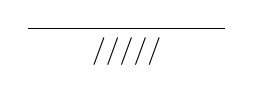
\begin{tikzpicture}
\draw[-,>=latex] (0.75, 0)--(3.25, 0) node[below left] {} ; 
\draw[] (2, 0)--(2, 0) node[below] {$/////$} ; %x_T
\end{tikzpicture}
\caption{}
\label{figb}
\end{subfigure}
%\hfill
\begin{subfigure}[b]{.3\linewidth}
\centering
\begin{tikzpicture}
\draw[-,>=latex] (0.75, 0) --(3.25, 0) node[below] {$/////$} ; 
\end{tikzpicture}
\caption{}
\label{figc}
\end{subfigure}
%\hfill
\hfill
\newline$\,$\\
\begin{subfigure}[b]{.3\linewidth}
\centering
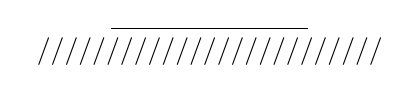
\begin{tikzpicture}
\draw[-,>=latex] (0.75, 0)--(3.25, 0) node[below left] {} ; 
\draw[] (2, 0)--(2, 0) node[below] {$/////////////////////////$} ; %x_T
\end{tikzpicture}
\caption{}
\label{figd}
\end{subfigure}
%\hfill 
\begin{subfigure}[b]{.3\linewidth}
\centering
\begin{tikzpicture}
\draw[white,-,>=latex] (0.5, 0)--(3.5, 0) node[below left] {} ; 
\draw[white] (2, 0.5)--(2, -0.1) node[below] {$//////$} ; %x_T
\end{tikzpicture}
%\subcaption*{fig.9}
\end{subfigure}
%\hfill
\begin{subfigure}[b]{.3\linewidth}
\centering
\begin{tikzpicture}
\draw[white,-,>=latex] (0.5, 0)--(3.5, 0) node[below left] {} ; 
\draw[white] (2, 0.5)--(2, -0.1) node[below] {$//////$} ; %x_T
\end{tikzpicture}
%\subcaption*{fig.9}
\end{subfigure}
\end{figure}  
 

 
I will now discuss the four scenarios in \figref{Fig6} one by one, providing evidence for each option.  


\subsubsection{Ingressive reading (Fig. \ref{Fig6}, sce. \subref{figa})}\label{ingr}
Scenario \subref{figa} shows the transfer from a time where the eventuality assigned to $e$ is not yet running to a time where it is running.
Accordingly, if we stick to sentences with a verb having the stem \textit{pis-}, the respective interpretation 
should amount to the onset of a writing. 

More often than not, however, the verb \textit{pisat'} by itself will not be found to express `start writing'. 
Instead, speakers use a phase verb plus an imperfective infinitive as its complement, as in \textit{načal pisat'}, or an ingressive prefix \textit{za-}, as in \textit{zakuril}:

\ea\label{orlov}
\gll Orlov načal pisat' pis'mo, a Grejg
zakuril svoju trubku ... \\
O. begin.\textsc{pst.pfv} write.\textsc{inf.ipfv} letter whereas G. 
start.smoke.\textsc{pst.pfv} 
\textsc{refl} pipe  \\
\glt `Orlov started writing a letter, and Grejg lighted his pipe ...' \hfill (NKRJa)
\z

\noindent Nevertheless, an ingressive reading for 
Russian 1-state verbs 
can be attested. In the following example, it is the verb 
\textit{plakat'} `to cry' that is used in this way.\footnote{Thanks to two reviewers for telling me that such examples do exist.} 

\ea\label{plakal}
\gll Menja posetilo takoe oščuščenie sčast'ja i
odnovremenno otčajanija, čto ja pribežal v artističeskuju, zapersja i  plakal.\\
me catch.up.\textsc{pst.pfv} such feeling luck and simultaneously 
desperation 
that I run.to.\textsc{pst.pfv} in backstage.room lock.\textsc{pst.pfv} 
and cry.\textsc{pst.ipfv} \\
\glt `I got such a feeling of luck and desperation that I ran to the backstage room, locked myself up and started to cry.' \hfill (NKRJa)
\z

%К моему удивлению, кот сразу же ел и сухой, и консервы (раньше пробовала Роял Канин, то отказывался)

\subsubsection{Progressive reading (Fig. \ref{Fig6}, sce. \subref{figb})}
DASP applying to (the meaning of InstP projected from) a 1-state predicate also generates scenario \subref{figb} as possible interpretation. 
This interpretation corresponds to what is usually called progressive reading.
The topic time is properly included in the time of the eventuality, giving rise to the internal viewpoint effect (see \citealt{Smith1991}). 
(\ref{orlov1}) shows an example:

\ea\label{orlov1}
\gll Džen
sidela na  kuchne i pisala ėlektronnoe pis'mo, kogda Mėtt prišel domoj s raboty.\\
J. sit.\textsc{pst.ipfv} in 
kitchen and write.\textsc{pst.ipfv} electronic letter
when M. come.\textsc{pst.pfv} home from work\\
\glt `Jane was sitting in the kitchen and was writing an email, when Matt came home from work.' \hfill (e-libra.ru)
\z

\noindent In this example, the topic time is supplied by the temporal clause,  corresponding to the run time of the event of Matt's coming home. This event is temporally included in the event of Jane's writing an email, thus instantiating the interpretation depicted in scenario \subref{figb} of \figref{Fig6}.

\subsubsection{Egressive reading (Fig. \ref{Fig6}, sce. \subref{figc})}\label{egr}
In scenario \subref{figc}, we encounter another relation between the topic time and the eventuality time that (\ref{boxaspdo}) allows for. 
Here, the topic time exceeds the right edge of the run time of the eventuality assigned to the discourse referent $e$.
An interpretation in line with this scenario will thus convey the message that the final stage of the eventuality
has been left behind. 
%The topic time interval accompanies a change from the existence of $e$ to its non-existence. 

This case represents the mirror image of \ref{ingr}. And just like in that case, Russian provides special means 
serving the function of expressing the interpretation relevant to the issue. 
For one thing, Russian makes systematic use of the phase verb \textit{končit'} `finish' in combination with
imperfective infinitives like, for instance, \textit{pisat'}. Moreover,
the completive prefix \textit{do-} may productively be used to form perfective verbs like \textit{dopisat'} `finish writing'.

Nevertheless, 1-state predicates may be used to convey the egressive reading in the appropriate setting. Witness the compatibility of the form \textit{čital} with \textit{do konca} `to the end'.\footnote{I thank a reviewer for bringing this up to me. In the first version of this chapter I held the view that the egressive interpretation of a simple imperfective would totally be blocked by the availability of the respective phase verb construction.}

\ea\label{dokonca}
\gll ...
a potom  už ne mog prervat' čtenie, čital do konca, sdelal liš' nebol'šoj pereryv, čtoby podkrepit'sja rjumočkoj.\\
{} and then already 
not can.\textsc{pst.ipfv} interrupt.\textsc{inf.pfv} reading read.\textsc{pst.ipfv} until end 
do.\textsc{pst.pfv} only small pause to draw.strength.\textsc{inf.pfv} vodka.shot\\
\glt `...and from then I could not stop reading, I read to the end, made only a small pause to regain energy by having a vodka.' \hfill (NKRJa)
\z
 
\subsubsection{General-factual reading (Fig. \ref{Fig6}, sce. \subref{figd})}
Last but not least, (\ref{boxaspdo}) allows for the interpretation \subref{figd} of \figref{Fig6}.
In this case, the topic time properly includes the whole time of the eventuality. 
Recall that we deal only with 1-state predicates in this section, so the eventuality has to be either a state or a process.  
This scenario implies two changes: the first leading from the non-existence of the eventuality to its existence, 
the second from its existence to its non-existence. 

The interpretation given in scenario \subref{figd} of \figref{Fig6} is well-attested.
It is referred to as the ``general-factual'' meaning 
in the traditional aspectological literature. (\ref{leninread}) shows an example discussed in \citet[343]{Paslawska.Stechow2003} (see \citealt[25]{zaliznjaksmelev97} for more examples):\footnote{In (\ref{leninmod}) I presented a variation of it. Note that, unlike the predicate \textit{read War and Peace}, the predicate \textit{read Lenin} is atelic (1-state).}

\ea\label{leninread}
\gll Vse sčitali ego obrazovannym čelovekom. On čital Lenina.  \\
everyone consider.\textsc{pst.ipfv} him 
educated person he  read.\textsc{pst.ipfv} Lenin\\
\glt `Everyone took him for a knowledgeable person. He had read Lenin.'
\z

\subsection{DASP applied to 2-state predicates}\label{dasptwo}

The previous section was about the spectrum of readings that DASP 
will give rise to when applying to the meaning of an InstP that is based on a 1-state predicate. Now I move on
to investigate the range of interpretations that DASP produces when it operates over 2-state meanings.  For the purpose of illustration, I will use the same example that I used above:
this section discusses the case of verbs having the stem \textit{podpis-},
\S \ref{daspthree} will be about verbs having the same stem prolonged by YVA, i.e. \textit{podpisyv-}. 

Processing InstP with [\textsubscript{VP} [\textsubscript{V} \textit{podpis-}] [\textsubscript{DP} [\textsubscript{D} $\emptyset$][\textsubscript{NP} \textit{pis'mo}]]] as VP will result in the DRS given in (\ref{boxpodinstdo}). To compute the meaning of AspP, we have to update it in line with the construction rule for DASP, (\ref{CRdasp}). The result is shown in (\ref{boxpodaspdoo}).

\eabox{\label{boxpodaspdoo}
\drs{t$_{top}$ e$_1$ e$_2$ z }{\textsc{sign}($e_1$) \\ \textsc{signed}($e_2$) \\ \cnst{cause}($e_1$,$e_2$) \\ \cnst{ovl}($e_{fin}$,$t_{top}$) \\ $e_2$ = $e_{fin}$ \\
\cnst{author}($e_1$,\d{$x$}) \\ \cnst{text}($e_1$,$z$) \\ \textsc{letter}($z$)}
}

\noindent Given (\ref{boxpodaspdoo}), the scenarios in \figref{Fig7} exhaust the range of interpretations that the verb \textit{podpisat'} may in principle give rise to.
They represent all of the logically possible
relations that the relation $\cnst{ovl}(e_2,t_{top})$ allows for
(the vertical line symbolizes the temporal point where $f(e_1$) and $f(e_2$) abut). 

\begin{figure}
\caption{\label{Fig7}possible scenarios for (\ref{boxpodaspdoo})}
\begin{subfigure}[b]{.3\linewidth}
\centering
$\,\,\,$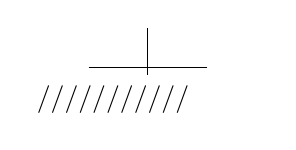
\begin{tikzpicture}
\draw[-,>=latex] (1.25, 0)--(2.75, 0) node[below left] {} ; 
\draw[] (2, 0.5)--(2, -0.1) node[below] {$///////////\textcolor{white}{/////}$} ; %x_T
\end{tikzpicture}
\caption{}
\label{sca}
\end{subfigure}
\begin{subfigure}[b]{.3\linewidth}
\centering
\begin{tikzpicture}
\draw[-,>=latex] (1.25, 0)--(2.75, 0) node[below left] {} ; 
\draw[] (2.0, 0.5)--(2.0, -0.1) node[below] {$/////$} ; %x_T
\end{tikzpicture}
\caption{}
\label{scb}
\end{subfigure}
\begin{subfigure}[b]{.3\linewidth}
\centering
\begin{tikzpicture}
\draw[-,>=latex] (1.25, 0)--(2.75, 0) node[below left] {} ; 
\draw[] (2, 0.5)--(2, -0.1) node[below] {$\quad\quad\,\,\,///\textcolor{white}{/}$} ; %x_T
\end{tikzpicture}
\caption{}
\label{scc}
\end{subfigure}
\newline$\,$\\
\begin{subfigure}[b]{.3\linewidth}
\centering
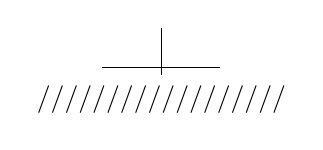
\begin{tikzpicture}
\draw[-,>=latex] (1.25, 0)--(2.75, 0) node[below left] {} ; 
\draw[] (2, 0.5)--(2, -0.1) node[below] {$//////////////////$} ; %x_T
\end{tikzpicture}
%\includegraphics[width=3.5cm]{anatomie1.jpg}
\caption{}
\label{scd}
\end{subfigure}
\begin{subfigure}[b]{.3\linewidth}
\centering
$\,\,$\begin{tikzpicture}
\draw[-,>=latex] (1.25, 0)--(2.75, 0) node[below] {} ; %x-Achse
%\draw[->,>=latex] (0, 0)--(0, 4) node[below left] {\(log(S)\)} ; %y-Achse
\draw[] (2, 0.5)--(2, -0.1) node[below] {$\quad\quad\,\,\,////////////$} ; %x_T
\draw[white] (3.5, 0.5)--(3.5, -0.1) node[below] {$/////$} ; %x_T
\end{tikzpicture}
\caption{}
\label{sce}
\end{subfigure}
\begin{subfigure}[b]{.3\linewidth}
\centering
$\,\,\,\,\,$\begin{tikzpicture}
\draw[-,>=latex] (1.25, 0)--(2.75, 0) node[below] {} ; 
\draw[] (2, 0.5)--(2, -0.1) node[below] {$\quad\quad\quad\,\,\,////$} ; %x_T
\draw[white] (3.5, 0.5)--(3.5, -0.1) node[below] {$/////$} ; %x_T
\end{tikzpicture}
\caption{}
\label{scf}
\end{subfigure}\hfill
\end{figure}

As before, I will now briefly discuss these configurations one by one. 

\subsubsection{Concrete-factual reading (Fig. \ref{Fig7}, sce. \subref{sca})}\label{cfr}
Following Russian aspectological tradition, I call the first reading to be discussed \textsc{concrete factual}. 
The content of this label is described in the Academy Grammar (\citealt[604]{Svedova1980}) 
as reference to a single situation presented as a 
concrete whole fact limited by a boundary
(``konkretnyj celostnyj fakt, ograničennyj predelom'').
This is just what is depicted in scenario \subref{sca} of \figref{Fig7}:
The ``whole fact'' corresponds to the full inclusion of the eventuality assigned to $e_1$
in the topic time. The ``limitation by a boundary'' corresponds to that the topic time ends within the time of the eventuality assigned to $e_2$, which implies a change from $f(e_1$) to
$f(e_2$). A classic example with three such changes forming a chain of events is given in (\ref{cesar}). 

\ea\label{cesar}
\gll Prišel,
uvidel, pobedil. \\
come.\textsc{pst.pfv} see.\textsc{pst.pfv} 
defeat.\textsc{pst.pfv}  \\
\glt `Veni, vidi, vici.' 
\z 

\subsubsection{Culmination-in-focus (Fig. \ref{Fig7}, sce. \subref{scb})}\label{trans}
The interpretation depicted in \figref{Fig7} as scenario \subref{scb} differs from scenario \subref{sca} (of \figref{Fig7}) in that the start of the eventuality assigned to $e_1$ precedes the start of the topic time interval.
Since the onset of the first eventuality lies outside of ``the time for which an assertion is made'' (\citealt[687]{Klein1995}), it will not fall within the scope of what the utterance is about.
%A verb which is interpreted in accordance with figure 6 will thus exclusively be about 
%the change from $e_1$ to $e_2$.
Such a reading, which I will call \textsc{culmination-in-focus} for lack of a better term,
is pragmatically licenced as an answer to an (implicit or explicit) 
question that queries whether $f(e_2$) has, or has not, been reached within $t_{top}$, presupposing that $f(e_1$) is running.
Imagine a situation where two friends are reading a book together, turning one page after the other. One is about to turn the next page. Here the following dialogue fits in (from \citealt[145]{Plungjan01}).\footnote{An anonymous reviewer points out that the theory seems to overgenerate at this point. In a context where Peter has been reading \textit{War and Peace} for months, and is already near the end, and the speaker thinks that Peter will finish it tomorrow, there is no culmination-in-focus interpretation available for \textit{Petja zavtra pročitaet ``Vojnu i mir''} (Peter tomorrow read-through War-and-Peace). Indeed, the correct form to convey the intended message would be \textit{dočitaet}. Completive \textit{do-} has a presuppositional meaning (described in \citealt{Kagan15}) which is well-suited for culmination-in-focus contexts. In such contexts, perfectives formed by means of \textit{do-} seem to win over perfectives formed by means of ``empty'' prefixes (like \textit{pro-} in \textit{pročitat'} or \textit{na-} in \textit{napisat'}). Why that should be so is an intriguing topic for future research.}

%\ea\label{plungraupe}
%\gll \textit{Vy} \textit{vdvoem} \textit{s} \textit{prijatelem} \textit{čitaete} \textit{ėtu} \textit{knigu,} \textit{perevoračivaja} \textit{stranicu} \textit{za} \textit{stranicej.} \textit{Prežde}  \textit{čem} \textit{odin} \textit{iz} \textit{vas} \textit{perevernet} \textit{stranicu,} \textit{on,} \textit{estestvenno,} \textit{sprašivaet} \textit{u} \textit{drugogo:} \textit{``Pročital?''}\\
%you two with friend read.\textsc{prs.ipfv} this book turning page for page before than one from you turn.\textsc{prs.pfv} page he of.course ask.\textsc{prs.ipfv} at other read.\textsc{pst.pfv}\\
%\glt \normalsize{`You and a friend are reading this book, turning one page after the other. Before one of you will turn the page, he will, of course, ask: Are you done (with reading)?'} 
%\z

%%Ну что прочитал Плунгян CHECK
\ea\label{raupe1}
\begin{itemize}
\item[A:] \gll Pročital?\\
read.\textsc{pst.pfv}\\
\glt `Are you done with reading?'
\item[B:] \gll Da, pročital.\\
yes read.\textsc{pst.pfv}\\
\glt `Yes, I am.' 
\end{itemize}
\z
%\ea\label{raupe}
%\gll \textit{V} 
%\textit{ėtu} \textit{noč',} \textit{bliže} \textit{k}
%\textit{rassvetu,} \textit{žena}
%\textit{blagopolučno} \textit{rodila} \textit{mal'čika.}  \\
%in that night closer to dawn wife felicitously \normalsize{give.birth.\textsc{pst.pfv}} boy \\ 
%\glt \normalsize{`In that night, at break of dawn, his wife naturally gave birth to a boy.'} \hfill (NKRJa)
%\z  
\noindent It should be noted that 
in the Russian Academy Grammar what I call culmination-in-focus here is grouped together with the reading in \S \ref{cfr} under the heading 
``konkretno-faktičeskij tip upotreblenija'' (\citealt[605]{Svedova1980}). The same holds for
the interpretation to be discussed in the next section, which is likewise treated as a special case of concrete-factual 
(see \citealt[606]{Svedova1980}).

\subsubsection{Perfect reading (Fig. \ref{Fig7}, sce. \subref{scc})}\label{perfect}
Scenario \subref{scc} of \figref{Fig7} shows the interpretation known as perfect reading (``perfektnoe značenie'').
What is characteristic of the perfect reading is that the moment of change to $f(e_2$) lies before the beginning of the topic time, and that the topic time ends when $f(e_2$) is still in force.
The respective utterance will accordingly be about the holding of the target state, i.e. the eventuality assigned to $e_2$. The following example is from \citet{Svedova1980}.

\ea\label{raupe2}
\gll On postarel, raspolnel i obrjuzg. \\
he grow.old.\textsc{pst.pfv} fatten.up.\textsc{pst.pfv} and bloat.\textsc{pst.pfv}\\ 
\glt `He is old, fat and bloated now.' 
\z 

\noindent Two things are worth noting with respect to (\ref{raupe2}).
For one thing, the example shows that perfectivity does not rule out the possibility that the topic time and the utterance time overlap (contra \citealt{Borik2006}). Moreover, the example also shows that perfectivity does not necessarily enforce a chain-of-events interpretation (contra to what is stated above in (\ref{diagd}), see also fn. \ref{kicker}).   

\subsubsection{Pluperfect readings (Fig. \ref{Fig7}, sce. \subref{scd}, \subref{sce}, and \subref{scf})}\label{plu}
Besides the interpretations discussed so far, DASP 
allows for three more options, depicted in \figref{Fig7} as the scenarios
 \subref{scd}, \subref{sce}, and \subref{scf}.
Also in these cases, an overlap of the topic time and the run time of the eventuality assigned to $e_2$ is warranted.
We observe systematic relationships:
\subref{scd} differs from \subref{sca} in that the right edge of the topic time goes beyond the end of the run time of $f(e_2$), and so differ \subref{sce} and \subref{scf} 
from \subref{scb} and \subref{scc}, respectively. Below, I argue that these interpretations
represent pluperfect, or past perfect, readings (\citealt[133]{Borik2006}).

%We noted that in these cases, the end of the eventuality assigned to e$_2$ falls inside the topic time. Accordingly, what figures 8--10 stand for are utterances not only about the event (by ``event'' I mean the eventuality consisting of $f(e_1)$ and $f(e_2)$), but also about something going on after it.  

Later on in the derivation, when the semantic contribution of T is calculated at TP, the topic time will be related to the time of the utterance. If the tense is past, the topic time interval should be located before the utterance time. Since this also includes the end of the topic time, the configurations \subref{scd}--\subref{scf} leave no room for the utterance time to fall within the time of the event. This is in contrast to the scenarios \subref{sca}--\subref{scc} where, under the past tense, the utterance time may be located after the end of the topic time within the time of $f(e_2)$. 

This dissociation of the eventuality time from the utterance time entails a transposition of the relevance center of the utterance, as the consequences of the change that the event describes, i.e. the conditions of $f(e_2)$, must now be understood as being relevant to some time prior to the utterance time. 
The scenarios depicted in \subref{scd}--\subref{scf} imply, in other words, a
secondary evaluation time for the event in addition to the ultimate evaluation time, which is the utterance time.   

\citet{Comrie1997} points out that speakers often use the phase particle \textit{uže} `already' together with a perfective verb in order to express pluperfect meanings, for which there is no specialized grammatical construction in Russian (see also \citealt[309]{Paslawska.Stechow2003}). This is not by chance.
The semantics of \textit{uže} is such that it contrasts two temporal phases with each other: a phase at which the relevant property
(the one delivered by the predicate with which the particle combines)
is asserted to hold, and a later phase at which the same property is presupposed to hold (see \citealt{Ippolito2007}).
Applied to our case, the relevant property is the condition of $f(e_2)$. 
With these conditions being presupposed (and thus expected) to hold at utterance time, it is asserted that they in fact, unexpectedly, 
held at some earlier time. 
This ``earlier time'' (the new evaluation time) is usually introduced by explicit linguistic material. In \citeposst{Paslawska.Stechow2003} example (\ref{8postpst}), for instance, it is explicated by the temporal adverbial \textit{v vosem' časov}:

\newpage
\ea\label{8postpst}
\gll V vosem' časov, Maša uže vyšla.  \\
in eight hours M. already go.out.\textsc{pst.pfv} \\
\glt `At eight, Masha had already left.'
\z

%\ea\label{cesar3}
%\gll ... \textit{v} \textit{1960} \textit{godu}
%\textit{mne} \textit{uže} \textit{ispolnilos'}
%\textit{dvadcat'} \textit{vosem'.}\\
%{} in 1960 year me already %\normalsize{fulfill.\textsc{pst.pfv}}  \normalsize{twenty} %\normalsize{eight}\\
%\glt \normalsize{`... in 1960 I had already reached the age %of 28.'} \hfill \textcolor{gray}{NKRJa}
%\z 

%What figures 8-10 express are, of course, pluperfect readings. 
\noindent While (\ref{8postpst}) illustrates the reading \subref{scd}, (\ref{cesar4}) exemplifies 
the reading \subref{sce} of \figref{Fig7}. This latter scenario is tantamount to the pluperfect version of the ``culimination-in-focus'' reading (\S \ref{trans}).

\ea\label{cesar4}
\gll Kogda vrač
prišel, ona uže
rodila. \\
when doctor come.\textsc{pst.pfv} 
she already give.birth.\textsc{pst.pfv} \\
\glt `When the doctor arrived, she had already given birth.' \hfill (babyblog.ru)
\z 

\noindent Here, the earlier evaluation time, relative to which the birth is interpreted, is supplied by the subordinate clause. 
Finally, (\ref{tennis}) shows a pluperfect construal of the perfect reading described in \S \ref{perfect}:   

\ea\label{tennis}
\gll V
2012 godu ja uže
ustala ot tennisa i rešila zakončit'.\\
in 2012 year I already get.tired.\textsc{pst.pfv} 
of tennis and decide.\textsc{pst.pfv} finish.\textsc{inf.pfv} \\
\glt `In the year 2012 I was already tired of tennis and decided to finish with it.' \hfill (sports.ru)
\z 

\noindent By uttering (\ref{tennis}), the speaker informs the hearer that she is tired of playing tennis 
and that this state was held earlier than the hearer presumably expected, namely already in 2012.  

\subsection{DASP applied to a 2-state-predicate with the second eventuality argument uninstantiated}\label{daspthree}
Recall from above (\S \ref{S2}) that I treat the secondary imperfective marker YVA as a determiner element, which imposes on the two thematic eventuality arguments of a 2-state predicate the constraint that only the first of these, the source state argument, will be substituted by a discourse referent.\footnote{In fact, that is only one of two meanings that YVA may have, see (\ref{wää}). For space reasons, I cannot explore the theoretical consequences of the second, pluralizing construction rule (\ref{boh1}) in this chapter. I will have to leave that for future research.}    

If V is realized by some form of the verbal lexeme \textit{podpisat'}, and if Inst is realized by YVA, the DRS which is constructed by resolving InstP (the verbal counterpart of DP in the nominal projection) will be (\ref{boxinst1}).
Now let DASP apply to (\ref{boxinst1}) to form the meaning of AspP. Recall that I propose in this chapter that DASP will be operative in \textit{every} full verbal projection in Russian.
The construction rule for DASP is stated in (\ref{CRdasp}). It will give us (\ref{boxaspyva}).

\eabox{\label{boxaspyva}
\drs{t$_{top}$ e$_1$ z }{\textsc{sign}($e_1$) \\ \textsc{signed}($e_2$) \\ \cnst{cause}($e_1$,$e_2$) \\ \cnst{ovl}($e_{fin}$,$t_{top}$) \\ $e_1$ = $e_{fin}$\\
\cnst{author}($e_1$,\d{$x$}) \\ \cnst{text}($e_1$,$z$) \\ \textsc{letter}($z$)}
}

\noindent Given this meaning, the relation between the topic time and the run time of the eventuality assigned to e$_1$ may manifest itself in one of the ways shown in \figref{Fig8}.

\begin{figure}
\caption{\label{Fig8}possible scenarios for (\ref{boxaspyva})}
\begin{subfigure}[b]{.3\linewidth}
\centering
\begin{tikzpicture}
\draw[-,>=latex] (1,0) -- (2,0)[solid] {} ; %x-Achse
\draw[-,>=latex] (2,0) -- (3.0,0)[dashed] node[below left] {} ; 
\draw[] (2, 0.5) --(2, -0.1) node[below] {$\textcolor{white}{/}/////\textcolor{white}{//////////////}$} ; %x_T
\end{tikzpicture}
\caption{}
\label{pica}
\end{subfigure}\hfill
\begin{subfigure}[b]{.3\linewidth}
\centering
\begin{tikzpicture}
\draw[-,>=latex] (1,0) -- (2,0)[solid] {} ; %x-Achse
\draw[-,>=latex] (2,0) -- (3.0,0)[dashed] node[below left] {} ; 
\draw[] (2, 0.5)--(2, -0.1) node[below] {$\textcolor{white}{/}///\textcolor{white}{///////}$} ; %x_T
\end{tikzpicture}
\caption{}
\label{picb}
\end{subfigure}\hfill
\begin{subfigure}[b]{.3\linewidth}
\centering
\begin{tikzpicture}
\draw[-,>=latex] (1,0) -- (2,0)[solid] {} ; %x-Achse
\draw[-,>=latex] (2,0) -- (3.0,0)[dashed] node[below left] {} ; 
\draw[] (2, 0.5)--(2, -0.1) node[below] {$/////$} ; %x_T
\end{tikzpicture}
\caption{}
\label{picc}
\end{subfigure}\hfill
\newline$\,$\\
\begin{subfigure}[b]{.3\linewidth}
\centering
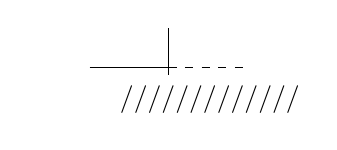
\begin{tikzpicture}
\draw[-,>=latex] (1,0) -- (2,0)[solid] {} ; %x-Achse
\draw[-,>=latex] (2,0) -- (3.0,0)[dashed] node[below left] {} ; 
\draw[] (2, 0.5)--(2, -0.1) node[below] {$\textcolor{white}{//////}/////////////$} ; %x_T
\end{tikzpicture}
\caption{}
\label{picd}
\end{subfigure}\hfill
\begin{subfigure}[b]{.3\linewidth}
\centering
\begin{tikzpicture}
\draw[-,>=latex] (1,0) -- (2,0)[solid] {} ; %x-Achse
\draw[-,>=latex] (2,0) -- (3.0,0)[dashed] node[below left] {} ; 
\draw[] (2, 0.5) --(2, -0.1) node[below] {$/////////////\textcolor{white}{///////}$} ; %x_T
\end{tikzpicture}
\caption{}
\label{pice}
\end{subfigure}\hfill
\begin{subfigure}[b]{.3\linewidth}
\centering
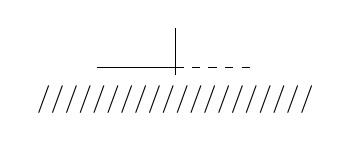
\begin{tikzpicture}
\draw[-,>=latex] (1,0) -- (2,0)[solid] {} ; %x-Achse
\draw[-,>=latex] (2,0) -- (3.0,0)[dashed] node[below left] {} ; 
\draw[] (2, 0.5) --(2, -0.1) node[below] {$////////////////////$} ; %x_T
\end{tikzpicture}
\caption{}
\label{picf}
\end{subfigure}\hfill
\end{figure}

In each of the scenarios of \figref{Fig8}, the topic time /// overlaps the run time of the eventuality assigned to the final discourse referent,
which, due to the impact of YVA, is now $e_1$. The dotted lines indicate that the respective target state argument $e_2$ is an implicit argument in (\ref{boxaspyva}). 

Just what does it mean for an argument to be implicit? \citet[61]{FarkasdeSwart2003} discuss example (\ref{vase}) in this regard. In that example, the implicit argument is the agent of the breaking event. 

 \ea\label{vase}
The vase was broken.
\z 

\noindent The authors propose that implicit arguments are represented by uninstantiated thematic arguments in final DRSs. As the final DRS for (\ref{vase}) they, accordingly, provide (\ref{vasedrs}).\footnote{\label{letters}\citet{FarkasdeSwart2003} use different letters for thematic arguments ($x$, $y$, $z$, ...) and discourse referents ($u$, $v$, $w$, ...). To not confuse the reader with too many different kinds of letters, I decided to use the same letters for thematic arguments and discourse referents in my semantic representations. Whether or not an argument is instantiated can unequivocally be told from whether or not it appears in $U_K$ (see footnote \ref{dots}).}

\eabox{\label{vasedrs}
\drs{u }{\cnst{vase}($u$) \\ \cnst{break}($x$,$u$)}
}

\noindent The reader who is familiar with standard DRT might want to object that the DRS (\ref{vasedrs}) is not proper because it seems to involve a free discourse referent $x$. This problem does not arise, however, as $x$ is not a discourse referent, but a thematic argument. Unlike discourse referents, thematic arguments are explicitly allowed to be free in final DRSs (\citealt[60]{FarkasdeSwart2003}). Of course, this modification of standard DRT calls for clarification of what it means for a condition involving a thematic argument to be verified in a model. To this end, \citet[63]{FarkasdeSwart2003} make the following proposal:

\eanoraggedright\label{verif}
Let $i$ be a variable over the elements in $\{1,\dots,n\}$. A function $f$ verifies a condition of the form $P(a_1,\dots,a_n)$ relative to a model $M$ iff there is a sequence $\langle e_1,\dots,e_n \rangle \in E^n$, such that $\langle e_1,\dots,e_n \rangle \in I(P)$, and if $a_i$ is a discourse referent, $e_i = f(a_i)$, and if $a_i$ is a thematic argument, $e_i$ is some element in~$E$.
\z

\noindent Following this example, I will assume that a DRS with an uninstantiated eventuality argument $e_2$ can be embedded if there is some element in E (the domain of entities in M) that corresponds to $e_2$. Importantly, nothing in definition (\ref{verif}) requires 
$f(e_2)$ to belong to the same world as $f(e_1)$.\footnote{Note a potential source of confusion: the letter ``$e$'' stands for entities in the model in (\ref{verif}), whereas in the main text it stands for elements in the DRS (thematic event arguments or discourse referents).} It is certainly true that the entity corresponding to the implicit argument $x$ in (\ref{vasedrs}), the agent of the breaking event, must live in the same world as the entity assigned to the discourse referent $u$, the broken vase. But this, I claim, is a pragmatic effect. It results from the fact that the existence of a consequent state (the vase being broken) presupposes the existence of a causing event (the breaking involving a causer) in the same world. In the cases of interest to us, the situation is different because of the flipped temporal order of the eventualities: the existence of a causing event (the signing of a document) does not presuppose the existence of a consequent state (the document being signed). The causing event may conceivably be interrupted half-way before it has caused the consequent state. (\ref{avarija1}) shows an attested example illustrating this case.          

\ea\label{avarija1}
\gll 
71-letnij akter v moment 
DTP perechodil ulicu, kogda na 
nego naechal avtomobil'.\\
71-year.old actor in moment accident cross.\textsc{pst.ipfv} street 
when on him drive.at.\textsc{pst.pfv} car \\
\glt `In the moment of the accident, the 71 year old actor was crossing the street  
when he was hit by a car.' \hfill (dni.ru)
\z 

\noindent So this is how the problem of the famous imperfective paradox (\citealt{Dowty1980,Landman92}) is addressed in the present approach.
Let us now look at the scenarios of \figref{Fig8} one by one.

 \subsubsection{Ingressive reading (Fig. \ref{Fig8}, sce. \subref{pica})}
In scenario \subref{pica} of \figref{Fig8}, we revisit the ingressive reading, this time based on a 2-state predicate.
Again, it should be noted that this reading is preferably expressed by means of the respective phase verb construction (e.g. \textit{načal otkryvat'}) or, however rare these cases may be, by ingressive \textit{za-} attaching to an otherwise imperfective base, as exemplified by \textit{zaotkryval} in (\ref{zaotkr}) (from \citealt[471]{Tate15}).

\ea\label{zaotkr}
\gll ... chrustnuli
rebra, vydavilsja 
poslednij vozduch iz legkich, i
mal'čiška zaotkryval
rot, kak ryba. \\ 
{} crack.\textsc{pst.pfv} ribs squeeze.out.\textsc{pst.pfv} final air from lungs and boy.\textsc{dim} start.open.\textsc{pst.pfv} mouth like fish \\
\glt `... ribs cracked, the last air was squeezed out of the lungs and the little boy started opening his mouth like a fish.' 
\z 

\noindent Besides that, one can also find attestations of bare 2-state imperfectives which are used in contexts where it is the onset of the event described that is at issue. Consider the following: it contains an imperfective verb morphologically derived from the otherwise perfective \textit{nasvistet'} `whistle a piece of music'.

\ea\label{plakal2}
%Он умылся, переоделся и насвистывал что-то веселое
\gll On umylsja, pereodelsja i nasvistyval čto-to veseloe.\\
he  wash.oneself.\textsc{pst.pfv} change.clothes.\textsc{pst.pfv} and whistle.\textsc{pst.ipfv} something cheerful\\
\glt `He washed himself, changed clothes and started to whistle something cheerful.' \hfill (NKRJa)
\z

\subsubsection{Progressive reading (Fig. \ref{Fig8}, sce. \subref{picb})}
Secondary imperfectives often actualize the progressive reading, represented in \figref{Fig8} by scenario \subref{picb}.
Recall from above that, due to the status of $e_2$ as an implicit/uninstantia\-ted argument, the verifying embedding for 
the final DRS built from (\ref{boxaspyva}) does not require the entities corresponding to $e_1$ and $e_2$ to belong to the same world. 

We already saw one example of the progressive reading in (\ref{avarija1}). Here is another one.  

 \ea\label{kontrakt}
\gll Kogda
ja podpisyval 
kontrakt, ja znal, čto
`Dinamo' nachoditsja daleko ne v 
lučšem položenii. \\
when I sign.\textsc{pst.ipfv} contract I know.\textsc{pst.ipfv} that D. is far not in best state \\
\glt `While I was signing the contract I knew that Dynamo was anything but in good condition.' \hfill (vtbrussia.ru)
\z 
 
\subsubsection{An impossible reading (Fig. \ref{Fig8}, sce. \subref{picc})} \label{sdfr}
Scenario \subref{picc} in \figref{Fig8} shows another way the topic time may overlap with the time of the eventuality assigned to $e_1$. I claim, however, that this configuration will never realize with secondary imperfectives, and here is why.

Note that the reading depicted in \subref{picc} wants the topic time to end within the time interval of the eventuality corresponding to $e_2$. This implies that the properties of the eventuality that is caused by $f(e_1)$ are of primary relevance to what the respective sentence conveys (\textit{target state relevance}, see \citealt{Gronn2004}). This is arguably not reconcilable with the fact that the argument of the caused eventuality is an implicit argument. To put it in a slogan: at-issue content should not be implicitly coded. 
Therefore, an accommodation process is activated:

\eanoraggedright \label{ttl}\textit{Derived instantiation} \\
If the topic time assigned to $t_{top}$ begins or ends within some eventuality corresponding to an argument in $Con_K$, that eventuality requires a discourse referent in $U_K$. If there is none, such a discourse referent will be accommodated.  
\z

\noindent Now see what this amounts to. After the accommodation of a discourse referent  $e_2$ in (\ref{boxaspyva}), the picture in \subref{picc} should be adjusted 
accordingly (the dotted line should be replaced by a straight line). What we end up with, then, is
the same interpretation as the one depicted in scenario \subref{scb} of \figref{Fig7} from above. Since scenario \subref{scb} of \figref{Fig7} is taken care of by the same verb
without secondary imperfective morphology, 
we arrive at a situation in which we have two candidate verbs for the same interpretation, \textit{podpisat'}
and \textit{podpisyvat'}. One of these is structurally more complex than the other. 
In such a situation, the pragmatic mechanism of \textit{morphological blocking} (\citealt{Kiparsky05, Deo2012}) will filter out the more complex 
expression.\footnote{This morphological blocking mechanism is often stated as an economy constraint saying that, all other things being equal, less complex expressions are preferred over more complex expressions
(e.g. \citealt{LeBruyn07}).}

Applied to our case, the impact of morphological blocking is that it will prevent secondary imperfectives 
from expressing the culmination-in-focus reading (scenario \subref{scb} of \figref{Fig7}). Being equivalent to scenario \subref{scb} of \figref{Fig7}, scenario \subref{picc} of \figref{Fig8} turns out to be no interpretive option
for verbs like, for instance, \textit{podpisyvat'}, \textit{vybrasyvat'} or \textit{otkryvat'}.\footnote{Looking at scenario \subref{picc} of \figref{Fig8}, a reviewer wonders whether my approach predicts secondary imperfectives to allow for the perfect reading. No, it does not. The perfect reading falls into the range of interpretative options for perfectives (see \S \ref{perfect}). Therefore, the use of the structurally more complex secondary imperfective in this function will also be ruled out by morphological blocking.}

\subsubsection{Annulment-of-result reading (Fig. \ref{Fig8}, sce. \subref{picd})}
Now let us consider \figref{Fig8}, scenario \subref{picd}. The topic time does not end within the time of the eventuality corresponding to $e_2$, but extends beyond its offset.\footnote{This is why (\ref{ttl}) does not apply.} If tense is past, the end of the target state eventuality must be understood as being located prior to the utterance time. So far, the interpretation depicted in this scenario matches the one of scenario \subref{sce} in \figref{Fig7}.

Moreover, a sentence expressing scenario \subref{picd} of \figref{Fig8} will never be about the whole complex event made up of one eventuality causing the other because the initial phase of the causing eventuality lies outside of the topic time. This is also in line with scenario \subref{sce} of \figref{Fig7}.

The crucial difference between scenario \subref{picd} of \figref{Fig8} and scenario \subref{sce} of \figref{Fig7} relates to the absence of a discourse referent for $e_2$ in the DRS generating the former, because the argument $e_2$ is an uninstantiated argument in (\ref{boxaspyva}). In \S \ref{sdfr} I stated that implicitly coded information can only have not-at-issue status.
So the question arises: Is there a way to understand a sentence that is about a caused state that is not at issue? Yes, there is. What one needs to do is to draw the implicature that the target state, which should belong to what the utterance is about, is cancelled within the limits of the topic time (%cf.
see \citealt[236]{Gronn2004}; see also \S \ref{gron}). This way, what the utterance is about is no longer the mere change from the source state to the target state, but rather the double change from the source state to the target state and again away from the target state.   
Of course, such an interpretation should be supported by the lexical semantics of the predicate (which should be such that the target state is cancellable under normal circumstances).   
I claim, in other words, that the reading of scenario \subref{picd} of \figref{Fig8} is attested by the much-discussed annulment-of-result imperfectives (see \citealt{Rassud68}, \citealt{paduceva96}).
%Here is an example, in addition to (\ref{someone}):
Recall (\ref{someone}) as an illustrative example. 
%\ea\label{sound}
%\gll \small{\textit{Otkryvali}} \textit{okno,} \textit{čtoby} \textit{vpustit'} \textit{svežij} \textit{vozduch.}\\
%\small{open.\textsc{pst.ipfv}} \small{window}  \small{to} \small{let.in.\textsc{pfv}} \small{fresh} \small{air} \\
%\glt \small{`We had opened the window to let in fresh air.'} \hfill \textcolor{gray}{www}
%\z 

\subsubsection{Another impossible reading (Fig. \ref{Fig8}, sce. \subref{pice})} 
In \figref{Fig8}, scenario \subref{pice} shares with scenario \subref{picc} the feature that the topic time ends within the interval of the caused eventuality, with the argument of the caused eventuality being uninstantiated. As argued in (\ref{ttl}), such a scenario calls for accommodation of a discourse referent $e_2$.
Since this will in effect make scenario \subref{pice} equivalent to scenario \subref{sca} of \figref{Fig7}, and since this latter interpretation is taken care of by a less complex verb (the same verb without secondary imperfective morphology),
scenario \subref{pice} of \figref{Fig8} turns out to be no interpretive option for a
secondary imperfective, due to morphological blocking.

\subsubsection{General-factual reading (Fig. \ref{Fig8}, sce. \subref{picf})}
The final reading to be discussed is shown in scenario \subref{picf} of \figref{Fig8}, which resembles scenario \subref{scd} of \figref{Fig7} in many respects.
Indeed, the two scenarios match in every detail, except for the way the information about the caused event is conveyed. 
In both cases, the topic time properly includes the intervals of the causing eventuality and the caused eventuality. 
The difference is that, while the argument $e_2$ of the DRS belonging to scenario \subref{scd} of \figref{Fig7} is instantiated, the argument $e_2$ of the DRS belonging to scenario \subref{picf} of \figref{Fig8} is uninstantiated.

Expecting that implicitly coded information provides not-at-issue content, we are entitled to draw the implicature that the specific conditions of the caused eventuality (target state) are irrelevant to the speaker's message. Since this is the core characteristics of general-factuals 
(\citealt[611]{Svedova1980}; \citealt{Gronn2004}), 
we arrive at the interpretation that we missed in \citeposst{Bohne2004} theory, i.e. the one which is expressed by sentences such as 
(\ref{blin}). 

What \textit{is} relevant instead of the target state conditions are the consequences of a rule in the background knowledge of the interlocutors, which is pragmatically pointed at by stating that an event of the respective kind has taken place. In (\ref{blin}), for instance, the relevant background rule follows from the fact that pancake recipes foresee only one flip of the pancake. Therefore, if a pancake has already been flipped, there is no need to do that again; see \citet{muellerhab} for more on the relevance of presupposed rules for general-factual interpretations. 

%Here is one more example ({\citealt[79-80]{Gronn2004}}):

%\ea\label{gronninterrupt}
%\gll \textit{Voobšče} \textit{ja} \textit{čital} \textit{``Vojnu i mir'', } \textit{chotja} \textit{po} \textit{pravde} \textit{ja} \textit{pročital} \textit{tol'ko} \textit{neskol'ko} \textit{stranic.}\\
%principally I read.\textsc{ipfv} {War and Peace} although after truth I read.\textsc{pfv} only some pages \\
%\trans `In principle, I've read \textit{War and Peace}. Though, to tell the truth, I've only read a few pages.'
%\z

%This example replicates the observation that I already mentioned in \ref{ssec:filip} with respect to (\ref{leinonen}): the information about event completion is cancellable in general-factuals. 
%This is explicable in terms of \citeposst{FarkasdeSwart2003} assumption (\ref{verif}), according to which implicit arguments require no more than that there is some suitable entity in the model.
%It follows from this liberal condition that the causing eventuality and the caused eventuality need not belong to the same world -- the existence of the causing eventuality in w does not entail the existence of the caused eventuality in w. Therefore, explicitly negating event completion, as in (\ref{gronninterrupt}), does not lead to a contradiction.  

% here Radek

\subsection{Briefly on external prefixation}\label{zapo}
The distinction between internal and external prefixes is well established in current research on the Slavic verb (see \S \ref{gr}). The most detailed stocktaking of Russian prefixation has probably been carried out in \citet{Tatevo13}. According to that study, external prefixes subclassify into left-peripheral, selectionally restricted, and positionally restricted prefixes. Here I can only scratch the surface and address selectionally restricted prefixes, in particular ingressive \textit{za-} and delimitative \textit{po-}. 

Selectionally restricted prefixes are so-called because of their limited combinatorics, as they successfully combine with an imperfective base only. The result of their application is a perfective.
Being aspect switchers, so to speak, they play a central role in the aspectual system of Russian. As pointed out by \citet{Dickey06}, they fill a systemic gap by deriving perfectives from atelic (or as I would say: 1-state) predicates.     

Following once again \citet{Ramchand08}, I treat Russian ingressive \textit{za-} and delimitative \textit{po-} as operating over the meaning of AspP, see (\ref{grza}). Note that the high application of external prefixes is essential to an analysis that considers perfective and imperfective meanings produced by DASP to be dependent on the presence or absence of state change.  

\subsubsection{Ingressive \textit{za-}}\label{zapoza}
Letting ingressive \textit{za-} apply after DASP only seems consequent in view of its selectional restriction to imperfective inputs. Its contribution of meaning may be stated in terms of the following construction rule:\footnote{$P$ stands for the property of the morphological base to which \textit{za-} attaches, the function $t_{init}(e)$ maps an eventuality onto its initial moment; the function $t_{fin}(e)$ maps an eventuality onto its final moment.}

\ea\label{CRza} Construction rule for ingressive \textit{za-} \\
- Introduce in $U_K$: a new eventuality discourse referent $e'$\\
- Introduce in $Con_K$: $\supset\subset (e',e)$\\
- Introduce in $Con_K$: \cnst{ovl}($t_{top},e'$)\\
- Introduce in $Con_K$: $\neg$ P($e'$)\\
- Introduce in $Con_K$: $\neg$ \cnst{ovl}($t_{top},t_{init}(e')$)\\
- Introduce in $Con_K$: $\neg$ \cnst{ovl}($t_{top},t_{fin}(e)$)\\
\z

\noindent Take a sentence whose VP is formed by the 1-state verb \textit{kuril} `he smoked'. According to what was said above, resolution of the AspP-node will give us the DRS (\ref{boxzap}). 

\eabox{\label{boxzap}
\drs{t$_{top}$ e }{\textsc{smoke}($e$) \\ \cnst{ovl}($e$,$t_{top}$) \\  \cnst{smoker}($e$,\d{$x$})}
}

\noindent Now let there be ingressive \textit{za-} attached as an adjunct to AspP. On account of the construction rule in (\ref{CRza}), the DRS resulting from processing the higher AspP \textit{zakuril} will look as follows:

\eabox{\label{boxzaplak}
\drs{t$_{top}$ e e'}{\textsc{smoke}($e$) \\ \cnst{ovl}($e$,$t_{top}$) \\  \cnst{smoker}($e$,\d{$x$})\\
$\supset\subset$ ($e'$,$e$)\\
\cnst{ovl}($t_{top}$,$e'$)\\
$\neg$ \textsc{smoke}($e'$)\\
$\neg$ \cnst{ovl}($t_{top}$,$t_{init}$($e'$))\\
$\neg$ \cnst{ovl}($t_{top}$,$t_{fin}$($e$)) }
}

\noindent This DRS will give rise to the readings depicted in \figref{radek}. Note that it is the second eventuality alone that satisfies the property described by the VP (due to condition ``$\neg$ smoke($e'$)''). The respective sentence is about a change from a situation of not smoking to a situation of smoking.
(\ref{orlov}) shows such a sentence. 
As we saw in (\ref{zaotkr}), moreover, ingressive \textit{za-} may also be used to prefix secondary imperfectives. This will give rise to an interpretation according to scenario \subref{radb}. 

\begin{figure}
\caption{\label{radek}possible scenarios for (\ref{boxzaplak})}
\begin{subfigure}[b]{.12\linewidth}
\centering
\begin{tikzpicture}
\draw[-,>=latex] (1.25, 0)--(2.75, 0) node[below left] {} ; 
\draw[] (2.0, 0.5)--(2.0, -0.1) node[below] {$/////$} ; %x_T
\end{tikzpicture}
\caption{}
\label{rada}
\end{subfigure}$\quad\quad\quad\quad$
\begin{subfigure}[b]{.2\linewidth}
\centering
\begin{tikzpicture}
\draw[-,>=latex] (1.25, 0)--(2.75, 0) node[below left] {} ; %x-Achse
\draw[-,>=latex] (2.75, 0)--(3.5, 0)[dashed] node[below left] {} ;
\draw[] (2.75, 0.5)--(2.75, -0.1) ;
\draw[] (2.0, 0.5)--(2.0, -0.1) node[below] {$/////$} ; %x_T
\end{tikzpicture}
\caption{}
\label{radb}
\end{subfigure}
\end{figure}

\subsubsection{Delimitative \textit{po-}}\label{zapopo}
The second selectionally restricted prefix that I want to discuss here is delimitative \textit{po-}.
(\ref{pokurilex}) shows a representative example. 

\ea\label{pokurilex}
\gll A ja vyšel, pokuril i vzjal
taksi. \\
and \textsc{1sg} go.out.\textsc{pst.pfv} smoke.a.bit.\textsc{pst.pfv} 
and take.\textsc{pst.pfv} taxi \\
\glt `And I went out, smoked a bit and took a taxi.' \hfill (NKRJa)
\z

\noindent To account for cases like \textit{pokuril} in (\ref{pokurilex}), 
I propose the following construction rule:

\ea\label{CRpo} Construction rule for delimitative \textit{po-} \\
- Introduce in $U_K$: a new eventuality discourse referent $e'$\\
- Introduce in $U_K$: a new eventuality discourse referent $e''$\\
- Introduce in $Con_K$: $\supset\subset (e',e)$\\
- Introduce in $Con_K$: $\supset\subset (e,e'')$\\
- Introduce in $Con_K$: \cnst{ovl}($t_{top},e'$)\\
- Introduce in $Con_K$: \cnst{ovl}($t_{top},e''$)\\
- Introduce in $Con_K$: $\neg$ P($e'$)\\
- Introduce in $Con_K$: $\neg$ P($e''$)\\
- Introduce in $Con_K$: $\neg$ \cnst{ovl}($t_{top},t_{init}(e')$)\\
- Introduce in $Con_K$: $\neg$ \cnst{ovl}($t_{top},t_{fin}(e'')$)\\
\z

\noindent Following the same procedure as above, the resolution of the first AspP-node will give us again (\ref{boxzap}). 
To this, we let delimitative \textit{po-} attach. The construction rule (\ref{CRpo}) will lead us to the meaning (\ref{boxpoplak}) for the higher AspP \textit{pokuril}:

\eabox{\label{boxpoplak}
\drs{t$_{top}$ e e' e''}{\textsc{smoke}($e$) \\ \cnst{ovl}($e$,$t_{top}$) \\  \cnst{smoker}($e$,\d{$x$})\\$\supset\subset$ ($e'$,$e$)\\ $\supset\subset $($e$,$e''$)\\
\cnst{ovl}($t_{top}$,$e'$)\\ \cnst{ovl}($t_{top}$,$e''$)\\
$\neg$ \textsc{smoke}($e'$)\\ $\neg$ \textsc{smoke}($e''$)\\
$\neg$ \cnst{ovl}($t_{top}$,$t_{init}$($e'$))\\
$\neg$ \cnst{ovl}($t_{top}$,$t_{fin}$($e''$))}
}

\noindent This DRS constrains possible interpretations to readings of the kind depicted in \figref{rit}.

\begin{figure}
\caption{\label{rit}possible scenarios for (\ref{boxpoplak})}
\begin{subfigure}[b]{.23\linewidth}
\centering
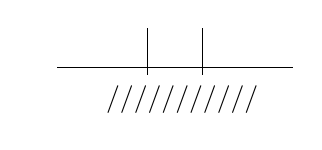
\begin{tikzpicture}
\draw[-,>=latex] (0.5, 0)--(3.5, 0) node[below left] {} ; 
\draw[] (1.65, 0.5)--(1.65, -0.1) node[below] {$\textcolor{white}{/////}///////////$} ; %x_T
\draw[] (2.35, 0.5)--(2.35, -0.1)  ; %x_T
\end{tikzpicture}
\caption{}
\label{rita}
\end{subfigure}
$\quad\quad\quad\quad$
\begin{subfigure}[b]{.3\linewidth}
\centering
\begin{tikzpicture}
\draw[-,>=latex] (0.5, 0)--(3.05, 0) node[below left] {} ; 
\draw[-,>=latex] (3.05, 0)--(4.2, 0)[dashed] node[below left] {} ; %x-Achse
%\draw[->,>=latex] (0, 0)--(0, 4) node[below left] {\(log(S)\)} ; %y-Achse
\draw[] (1.65, 0.5)--(1.65, -0.1) node[below] {$\textcolor{white}{/////}///////////$} ; %x_T
\draw[] (2.35, 0.5)--(2.35, -0.1)  ; 
\draw[] (3.05, 0.5)--(3.05, -0.1)  ;%x_T
\end{tikzpicture}
\caption{}
\label{ritb}
\end{subfigure}
\end{figure}

As can be seen, we arrive at an analysis that treats \textit{po}-delimitatives as expressing two subsequent changes, with the intermediate eventuality falling under the description of the 1-state predicate to which the prefix attaches. Such an analysis of Russian \textit{po}-delimitatives as expressing ``3-state-contents'' is not new. It has been proposed before by \citet[313--314]{Shatun09}. 

Delimitative \textit{po-} may also apply to secondary imperfectives, on condition that the eventuality leading to the state change (i.e. $f(e_1)$) is homogeneous (see \citealt{Mehlig06} for details). This results in the reading depicted in scenario \subref{ritb} of \figref{rit}.  

\subsubsection{Loose ends}\label{others}

Besides positionally-restricted and left-peripheral prefixations, I also ignore other selectionally-restricted prefixes noted by \citet[49]{Tatevo13}, such as distributive \textit{pere-} and cumulative \textit{na-}. Since their semantic impact goes beyond the manipulation of temporal relations, it is more complicated to state appropriate construction rules for these prefixations. So I refrain from doing that here, but I want to mention egressive \textit{ot-}, the antipode of ingressive \textit{za-}. Consider (\ref{otym}), which is among the top ten phrases of 2020 in Russia.\footnote{https://echo.msk.ru/blog/epsht.m/2759832-echo/} In this example, egressive \textit{ot-} attaches to the state verb \textit{imet'} `have'. The resulting perfective \textit{otymet'} describes a change from having something to not having something.   

\ea\label{otym}
\gll \v{Z}izn' otymela smysl. \\
life cease.to.have.\textsc{pst.pfv} sense \\
\glt `Life no longer makes sense.' 
\z 
  
\noindent The interpretation of this sentence will look like scenario \subref{rada} of \figref{radek},
whereby this time it is the first eventuality alone that satisfies the property of the base, P:

\ea\label{CRot} Construction rule for egressive \textit{ot-} \\
- Introduce in $U_K$: a new eventuality discourse referent $e'$\\
- Introduce in $Con_K$: $\supset\subset (e,e')$\\
- Introduce in $Con_K$: \cnst{ovl}($t_{top},e'$)\\
- Introduce in $Con_K$: $\neg$ P($e'$)\\
- Introduce in $Con_K$: 
$\neg$ \cnst{ovl}($t_{top},t_{init}(e)$)\\
- Introduce in $Con_K$: $\neg$ \cnst{ovl}($t_{top},t_{fin}(e')$)\\
\z

\noindent Let me end by pointing to a problem that my way of treating selectionally-restric\-ted (SR) prefixes faces.  
It is well-known that many perfectives that are derived that way (i.e. by attachment of a SR-prefix)
do not undergo secondary imperfectivization. This is, so far, in line with the theory presented above in which YVA applies before DASP and SR-prefixes apply after DASP. There are, however, also cases where SR-prefixes do allow for secondary imperfectivization, contra to what my analysis is predicting. Prominent examples are \textit{zapevat'} `start singing' and \textit{zakurivat'} `start smoking'. According to \citet{Zaliznjaketal2015}, the possibility of deriving such imperfectives increases with the frequency of the respective perfective. Given this, I am tempted to argue that in cases like \textit{zapevat'} or \textit{zakurivat'}, 
the respective prefixed verb has been lexicalized, i.e. reinterpreted by speakers as an instance of lexical prefixation. But this certainly deserves more exploration.

\subsection{Summary}\label{summo}
Above, I presented a theory that links verb forms to
the range of aspectual interpretations that they can actualize in Russian texts. In that approach, a single zero operator manages to correctly distribute perfective and imperfective forms among contexts.

The focus of the analysis was on the lexical stage of Russian verb formation, the domain of  
lexical/internal prefixes, and so-called secondary imperfective suffixes. In the end, I added some discussion of selected external prefixes. I gave a DRT-analysis in which verbal prefixes and suffixes do not by themselves express perfective or imperfective meanings (semantic aspects). Instead, these affixes are used to prepare, so to speak,
the input of the aspect operator. To this end, the story told is in line with conclusions drawn in works such as, inter alia, \citet{Filip2003} or \citet{Tate17}. 

The aspect operator DASP is conceived of, in the spirit of \citet{Klein1994}, as establishing a relation between topic time and eventuality time.
DASP is stated such that the eventuality assigned to the final discourse referent has to overlap topic time. Crucial is the assumption that secondary imperfective YVA marks the second argument of a 2-state predicate as an implicit argument, meaning that it has no discourse referent on its own. 

This gives us precisely what we observe: 2-state predicates without secondary imperfective morphology yield perfective meanings, 
while 1-state predicates and 2-state predicates with secondary imperfective morphology yield imperfective meanings. 
``Perfective meanings'' are meanings where the utterance is about the conditions of the instantiated target state. 
In the canonical case the topic time ends when the target state is in force (\textit{target state validity}, see \citealt{Gronn2004}). A variation on the theme are 
pluperfect readings, where the part of the topic time 
that goes beyond the end of the target state is dislocated from the utterance time. ``Imperfective meanings''
are all those meanings that do not entail target state validity. 

As for external prefixes like delimitative \textit{po-} or ingressive \textit{za-}, I have proposed that these come into play after DASP has applied (in line with \citealt{Ramchand2004, Ramchand08}). One might want to call this the second (syntactic) cycle of Russian verb formation. Accordingly, the semantics of these prefixes has to be stated such that they apply to already ``aspectualized'' meanings. 
%(cf. \citealt[1707]{Ramchand08}). 
These operators, in other words, take the output of DASP as input, mapping properties of times onto properties of times. Their output is a perfective meaning inasmuch as the topic time is required to end within the time of the final instantiated eventuality.   


\section*{Acknowledgements}
I wish to thank Berit Gehrke, Radek \v{S}im\'ik and three anonymous reviewers for their very helpful comments.
Many of the thoughts expressed here are the product of extremely constructive discussions with Hana Filip. 
I am also grateful to the audiences at the conference Formal Approaches to Russian Linguistics 3 (2019, Moscow State University), and at the Slavicus Expert Meeting on Aspect in Slavic (2022, University of Wroc\l{a}w) for criticism and comments. Special thanks go to: Daniel Altshuler, Hanna Bazanava, Petr Biskup, Marcel B\"orner, Tom Elvins, Dorota Klimek-Jankowska, Serge Minor, Michael M\"uller, Gillian Ram\-chand, Bo\.{z}ena Rozwadowska, Iuliia Shcherbina, Yulia Sorokina, Maria Su\-li\-mo\-va, Sergei Tatevosov, Marcin W\k agiel, Yulia Zinova, Karolina Zuchewicz. 
This chapter was submitted in February 2020. I regret that work published after that date, including my own, could not be considered. 


\section*{Abbreviations}

\begin{tabularx}{.5\textwidth}{@{}lX@{}}
\textsc{1}&1st person\\
\textsc{acc}&accusative\\
\textsc{dat}&dative\\
\textsc{dim}&diminutive\\
\textsc{gen}&genitive\\
\textsc{imp}&imperative\\
\end{tabularx}%
\begin{tabularx}{.5\textwidth}{@{}lX@{}}
\textsc{inf}&infinitive\\
\textsc{ipfv}&imperfective\\
\textsc{pfv}&perfective\\
\textsc{pst}&past\\
\textsc{refl}&reflexive pronoun\\
\textsc{sg}&singular\\
% &\\ % this dummy row achieves correct vertical alignment of both tables
\end{tabularx}



\sloppy
\printbibliography[heading=subbibliography,notkeyword=this]

\end{document}

